%% LyX 2.3.2 created this file.  For more info, see http://www.lyx.org/.
%% Do not edit unless you really know what you are doing.
\documentclass[12pt,english,titlepage, captions=tableheading, bibliography=totoc, usenames, dvipsnames]{scrartcl}
\usepackage{lmodern}
\renewcommand{\sfdefault}{lmss}
\renewcommand{\ttdefault}{lmtt}
\usepackage[T1]{fontenc}
\usepackage[latin9]{inputenc}
\setlength{\parskip}{\medskipamount}
\setlength{\parindent}{0pt}
\usepackage{color}
\definecolor{note_fontcolor}{rgb}{0, 0, 1}
\usepackage{babel}
\usepackage{booktabs}
\usepackage{textcomp}
\usepackage{enumitem}
\usepackage{amsmath}
\usepackage{graphicx}
\PassOptionsToPackage{version=3}{mhchem}
\usepackage{mhchem}
\usepackage[unicode=true,
 bookmarks=true,bookmarksnumbered=true,bookmarksopen=true,bookmarksopenlevel=2,
 breaklinks=false,pdfborder={0 0 1},backref=false,colorlinks=true]
 {hyperref}
\hypersetup{
 pdfauthor={Uwe St�hr},
 linkcolor=black, citecolor=black, urlcolor=blue, filecolor=blue, pdfpagelayout=OneColumn, pdfnewwindow=true, pdfstartview=XYZ, plainpages=false}

\makeatletter

%%%%%%%%%%%%%%%%%%%%%%%%%%%%%% LyX specific LaTeX commands.
\newcommand{\noun}[1]{\textsc{#1}}
%% Because html converters don't know tabularnewline
\providecommand{\tabularnewline}{\\}
%% The greyedout annotation environment
\newenvironment{lyxgreyedout}
  {\textcolor{note_fontcolor}\bgroup\ignorespaces}
  {\ignorespacesafterend\egroup}

%%%%%%%%%%%%%%%%%%%%%%%%%%%%%% Textclass specific LaTeX commands.
\newlength{\lyxlabelwidth}      % auxiliary length 

%%%%%%%%%%%%%%%%%%%%%%%%%%%%%% User specified LaTeX commands.
% Formatierung von Legenden
\usepackage[labelfont={bf,sf}]{caption}[2004/07/16]

% erm�glicht das Berechnen von Werten
\usepackage{calc}

%Vergr��ert den Teil der Seite, in dem Gleitobjekte
% unten angeordnet werden d�rfen
\renewcommand{\bottomfraction}{0.5}

% Vermeidet, dass Gleitobjekte vor ihrem Abschnitt gedruckt werden
\let\mySection\section\renewcommand{\section}{\suppressfloats[t]\mySection}

% Setzt den Link fuer Spruenge zu Gleitabbildungen
% auf den Anfang des Gelitobjekts und nicht aufs Ende
\usepackage[figure]{hypcap}

% Linkfl�che f�r Querverweise vergr��ern und automatisch benennen,
\AtBeginDocument{\renewcommand{\ref}[1]{\mbox{\autoref{#1}}}}
\AtBeginDocument{%
 \renewcommand*{\equationautorefname}[1]{}
 \renewcommand{\sectionautorefname}{sec.\negthinspace}
 \renewcommand{\subsectionautorefname}{sec.\negthinspace}
 \renewcommand{\subsubsectionautorefname}{sec.\negthinspace}
 \renewcommand{\figureautorefname}{Fig.\negthinspace}
}

% the pages of the TOC is numbered roman
% and a PDF-bookmark for the TOC is added
\let\myTOC\tableofcontents
\renewcommand\tableofcontents{%
  \pdfbookmark[2]{\contentsname}{}
  \myTOC
  \newpage}

% used to have extra space in table cells
\@ifundefined{extrarowheight}
 {\usepackage{array}}{}
\setlength{\extrarowheight}{2pt}

% color table cells
\usepackage{colortbl}

% enable comma as decimal separator
\usepackage{icomma}

% increase formula line separation
\setlength{\jot}{2mm+3pt}

\@ifundefined{showcaptionsetup}{}{%
 \PassOptionsToPackage{caption=false}{subfig}}
\usepackage{subfig}
\makeatother

\begin{document}
\title{Theory of RF-plasma processes}
\author{Uwe St�hr, Ph.D.\\
\\
Version 1.0}

\maketitle
\tableofcontents{}

\section{Plasma Frequency\label{sec:Plasma-Frequency}}

The plasma frequency $\omega_{e}$ is the eigenfrequency of the electrons.
Without external forces they oscillate with this frequency around
the ions. The derivation is simple: Assuming the electrons are shifted
by a length $x$ away from their position. The equation of motion
is then
\begin{equation}
m_{e}\ddot{x}=-eE\label{eq:motion}
\end{equation}
where $m_{e}=9.1\cdot10^{-31}\,$kg is the electron mass, $e=1.602\cdot10^{-19}\,$As
the elementary charge and $E$ the electric field strength.

Using the electron density $n_{e}$ in the \noun{Gauss} law we get
\begin{equation}
E=\frac{en_{e}}{\epsilon_{0}}\,x\label{eq:E-frequency}
\end{equation}
where $\epsilon_{0}=8.854\cdot10^{-12}\,$As/Vm is the vacuum permittivity.
Putting (\ref{eq:E-frequency}) into (\ref{eq:motion}) gives
\begin{equation}
0=\underbrace{\frac{e^{2}n_{e}}{m_{e}\epsilon_{0}}}_{\mathrm{eigenfrequency}}\,x+\ddot{x}
\end{equation}
Out of this oscillation equation we can directly read the expression
for the eigenfrequency:
\begin{equation}
\omega_{e}=\sqrt{\frac{e^{2}n_{e}}{m_{e}\epsilon_{0}}}
\end{equation}

Similarly to $\omega_{e}$ the eigenfrequencies for the ions can be
determined:
\begin{equation}
\omega_{i}=\sqrt{\frac{e^{2}n_{i}}{M\epsilon_{0}}}\label{eq:ion-plasma-frequency}
\end{equation}
where $M$ is the mass of an ion. Due to the global quasi-neutrality
$n_{e}\approx n_{i}$ for normal plasmas.

For a \href{https://en.wikipedia.org/wiki/Capacitively_coupled_plasma}{capacitively coupled plasma}
(CCP) RF-discharge at a pressure of a few pascals the typical electron
density is in the range of $10^{16}\,$1/m\textthreesuperior . This
leads to $\omega_{e}=5.6\,$GHz. For $\text{\ensuremath{O_{2}^{-}}}$-ions
with $M=5.312\cdot10^{-26}\,$kg we then have $\omega_{i\,\text{\ensuremath{O_{2}^{-}}}}=23.36\,$MHz.

\section{Plasma Sheath}

The sheath is the zone above the electrode and the chamber wall surface
where the electron density $n_{e}$ is much lower than the ion density
$n_{i}$. This zone is also visible as the ``dark zone'' when looking
into the chamber when a plasma is burning. The reason for the sheath
is that the RF of $f=\omega/2\pi=13.56\,$MHz is greater than the
ion plasma frequency $\omega_{i}$ but below the electron plasma frequency
$\omega_{e}$. Therefore the electrons can follow the electrical field
while the ions cannot.\footnote{\textbf{Note: }Hydrogen atoms are light enough to follow the electrical
field: $\omega_{H^{+}}\approx132\,$MHz.} So at the time where the electrode is positively charged, electrons
can stream out of the plasma to the electrode so that there is a region
where $n_{e}\approx0$ while $n_{i}\gg n_{e}$. The density distribution
at the electrode/walls is schematically shown in \ref{fig:Scheme-sheath}.

\begin{figure}[h]
\begin{centering}
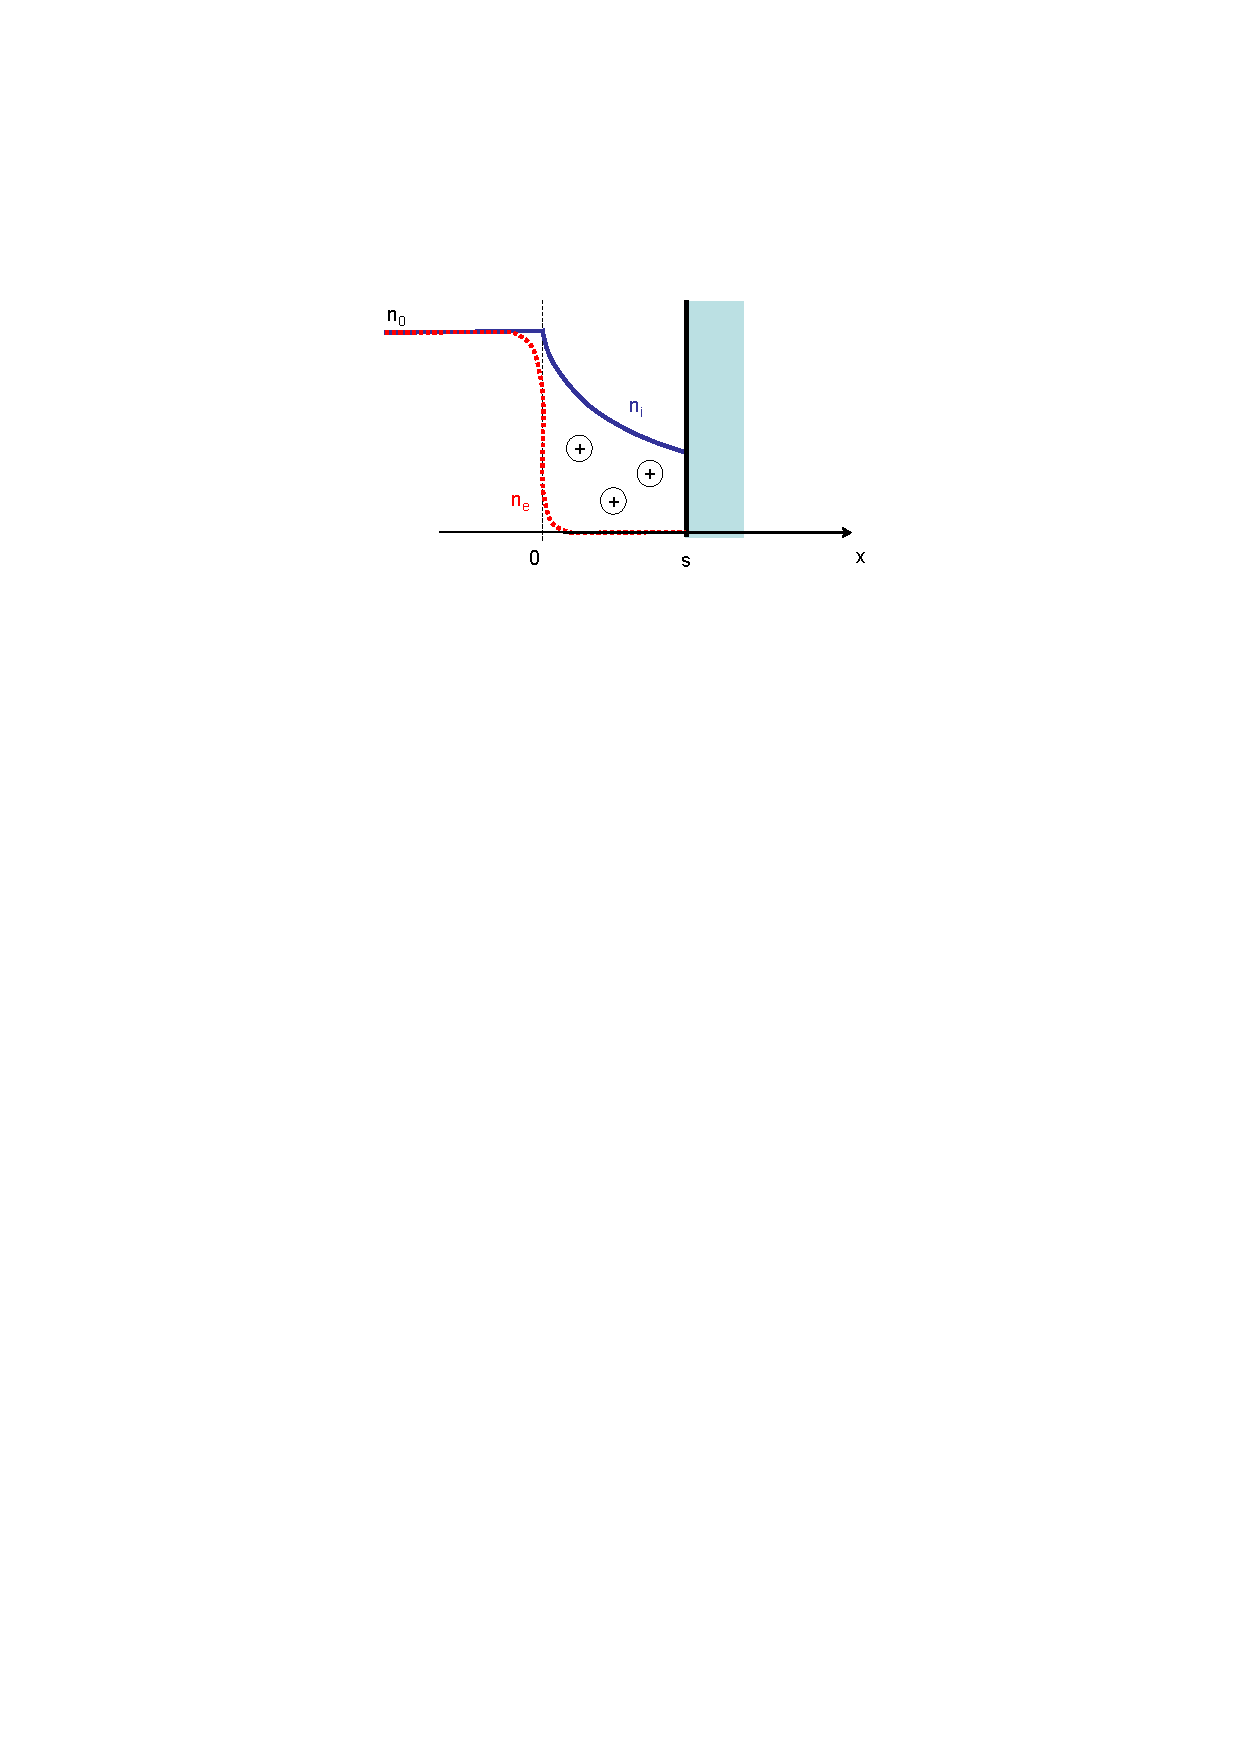
\includegraphics[width=0.5\columnwidth]{clipart/Sheath-scheme}
\par\end{centering}
\caption{\label{fig:Scheme-sheath}Scheme of the particle densities in a sheath.
The wall is at $x=s$, the sheath in the range $0\le x\le s$. Image
from \cite{Keudell12}.}
\end{figure}

The thickness of the sheath is important to know because it determines
the distance from the wall in which no substrates can be placed in
for coating. It also helps to approximate the dimensions of holes
and recessed areas in which strong plasma discharges will burn (hollow
cathode effect). This topic is discussed in \ref{sec:Hollow-cathode-effect}.

\subsection{Requirements for a Sheath}

What is necessary to get a sheath? It is known that there is no plasma
burning in small holes, so obviously there is not enough space to
form a sheath. The reason could be that the ions cannot be accelerated
to reach a level to build up the positive potential at the wall. That
this is indeed the reason is shown in the following.

The energy conservation leads to
\begin{equation}
E(x)=\frac{Mv_{i}^{2}(x)}{2}+e\,\varPhi(x)=\frac{Mv_{0}^{2}}{2}=E_{0}\label{eq:energy-conservation}
\end{equation}
where $M$ is the mass of an ion, $E(x)$ is the electric field strength
in the sheath, $\varPhi(x)$ the potential in the sheath, $v_{i}(x)$
the velocity of the ions in the sheath and $v_{0}$ the velocity of
the ions in the plasma bulk streaming into the sheath.

The charge also needs to be conserved so that the current $I$ through
the area $A$ of the sheath needs to be constant:
\begin{eqnarray}
\frac{I_{i}}{A} & = & \frac{I_{0}}{A}=\frac{N_{0}\cdot e}{tA}=n_{o}\cdot e\cdot v_{0}\\
n_{i}(x)v_{i}(x) & = & n_{0}v_{0}\label{eq:current-conservation}
\end{eqnarray}
($N$ is the number of particles and $t$ the time.) Putting (\ref{eq:current-conservation})
into (\ref{eq:energy-conservation}) we get
\begin{equation}
n_{i}(x)=n_{0}\,\left(1-\frac{e\,\varPhi(x)}{E_{0}}\right)^{-1/2}
\end{equation}
The plasma frequency of electrons is above the applied RF so that
they can follow this frequency. Therefore their density follows the
\noun{Boltzmann} relation:\footnote{See \cite[sections 2.2.4 and 2.2.5]{Keudell12-2} for a detailed derivation
of the \noun{Boltzmann} relation.}
\begin{eqnarray}
en_{e}\nabla\varPhi(x) & = & \nabla p(x)=\nabla n_{e}(x)k_{B}T\\
\frac{\mathrm{d}n_{e}(x)}{n_{e}(x)} & = & \frac{e\,\mathrm{d}\,\varPhi(x)}{k_{B}T_{e}}\\
n_{e}(x) & = & n_{0}\exp\left(\frac{e\,\varPhi(x)}{k_{B}T_{e}}\right)
\end{eqnarray}
with the \noun{Boltzmann} constant $k_{B}=1.38\cdot10^{-23}\,$J/K.

The \noun{Gauss} law is then
\begin{eqnarray}
\frac{\mathrm{d}^{2}\varPhi(x)}{\mathrm{d}x^{2}} & = & \frac{e}{\epsilon_{0}}\left(n_{e}(x)+n_{i}(x)\right)\label{eq:Gauss-law1}\\
 & = & \frac{en_{0}}{\epsilon_{0}}\,\left(\exp\left(\frac{e\,\varPhi(x)}{k_{B}T_{e}}\right)+\left(1-\frac{e\,\varPhi(x)}{E_{0}}\right)^{-1/2}\right)
\end{eqnarray}
($\epsilon_{0}$ is the vacuum permittivity.) It cannot be solved
analytically. For a derivation of an approximation at $\varPhi(x\approx0)$
see \cite[sec. "Raumladungszone einer Ionenrandschicht"]{Keudell12}.
This approximation delivers the relation
\begin{eqnarray}
\frac{\left(e\,\varPhi(x)\right)^{2}}{k_{B}T_{e}}-\frac{\left(e\,\varPhi(x)\right)^{2}}{2E_{0}} & > & 0\nonumber \\
\underbrace{\sqrt{\frac{k_{B}T_{e}}{M}}}_{v_{B}} & < & v_{0}\label{eq:Bohm-velocity}
\end{eqnarray}
$v_{B}$ is named \noun{Bohm} velocity and is the velocity that ions
must at least have so that a sheath can be formed. This velocity is
also the speed of sound of the ions.

\subsection{Mean Thickness of Sheaths}

We are working in a low pressure regime so that we can assume that
the mean free path $\lambda$ of the particles is independent of the
location in the plasma chamber. For the ion collision frequency we
can now write $\nu=\cfrac{v_{i}}{\lambda}$. With the ion velocity
$v_{i}(x)=\mu E(x)$, the ion drift mobility $\mu=\cfrac{e}{M\nu}$
and the field strength $E$ we can write
\begin{eqnarray}
v_{i}(x) & = & \frac{e\lambda}{Mv_{i}(x)}\,E(x)\nonumber \\
 & = & \sqrt{\frac{e\lambda}{M}\,E(x)}
\end{eqnarray}
where $M$ is the mass of an ion and $e$ the electron charge. The
ion density can now be calculated according to (\ref{eq:current-conservation}):
\begin{equation}
n_{i}(x)=\frac{v_{B}}{v_{i}(x)}\,n_{0}\label{eq:n_i}
\end{equation}
where $v_{B}$ is the \noun{Bohm} velocity that is necessary to get
a sheath, $T_{e}$ the electron temperature, $k_{B}$ the \noun{Boltzmann}
constant and $n_{0}\approx n_{e}\approx n_{i}$ the density in the
plasma bulk.

The simplest model of a sheath is that the electron density in the
sheath is zero. Using this we can neglect the electron density $n_{e}$
in the \noun{Gauss} law:
\begin{eqnarray}
\epsilon_{0}\,\frac{\mathrm{d}E}{\mathrm{d}x} & = & e\,\left(n_{i}(x)+\underbrace{n_{e}(x)}_{\approx0}\right)=\cfrac{e\,n_{0}\,\sqrt{\cfrac{k_{B}T_{e}}{M}}}{\sqrt{\frac{e\lambda}{M}\,E}}\label{eq:Gauss-law2}\\
\epsilon_{0}\sqrt{E}\,\mathrm{d}E & = & en_{0}\,\sqrt{\cfrac{k_{B}T_{e}}{e\lambda}}\,\mathrm{d}x=j_{0}\,\sqrt{\cfrac{M}{e\lambda}}\,\mathrm{d}x\label{eq:current-density}
\end{eqnarray}
($\epsilon_{0}$ is the vacuum permittivity and $j_{0}$ the current
density.) We integrate from the border of the sheath at $x=0$ to
the chamber border at $x=s$:
\begin{equation}
E^{3}=\frac{9}{4}\,s^{2}\,n_{0}^{2}\,\frac{e\,k_{B}T_{e}}{\epsilon_{0}^{2}\lambda}\label{eq:E-sheath}
\end{equation}
At the electrode we apply the voltage $U$ so that we have $E(s)=\cfrac{U}{s}$.
We can now calculate the sheath thickness $s$ to
\begin{equation}
s=\left(\frac{4U^{3}\epsilon_{0}^{2}\lambda}{9n_{0}^{2}ek_{B}T_{e}}\right)^{1/5}\label{eq:sheath-thickness}
\end{equation}
Using the relation for the mean free path assuming a \noun{Maxwell}
distribution for the molecule energies 
\begin{equation}
\lambda=\cfrac{k_{B}T}{\sqrt{2}\pi d^{2}p}\label{eq:lambda}
\end{equation}
($d$ is the diameter of the gas molecules.) (\ref{eq:sheath-thickness})
can be transformed to
\begin{equation}
s=\left(\frac{4U^{3}\epsilon_{0}^{2}T}{9\sqrt{2}n_{0}^{2}\pi epd^{2}T_{e}}\right)^{1/5}\label{eq:s-mean}
\end{equation}

The values for $\lambda$ for different precursors are listed in \ref{sec:Mean-Free-Paths}.
The mean voltage $\bar{U}$ at the electrode is the bias voltage so
that this can be used to calculate the mean sheath thickness $s$.

Taking typical values: $\lambda_{\ce{O2}}(p=2\,\mathrm{Pa})\approx8\,$mm,
$T\approx300\,$K, $T_{e}\approx3\cdot10^{4}\,$K, $n_{0}\approx10^{16}\,$1/m\textthreesuperior ,
$p=2\,$Pa, $\bar{U}\approx400\,$V leads with (\ref{eq:sheath-thickness})
to $s\approx4.7\,$mm.

(\ref{eq:s-mean}) is the time-independent mean sheath thickness where
also the dependency on the electrode area is not taken into account.
An approximation of a time- and area-dependent sheath thickness is
derived in the following section.

\subsection{Time-dependent Thickness of Sheaths}

A CCP is kept burning by shifting the charge within the chamber in
the applied frequency $\omega_{\mathrm{RF}}$. This displacement current
$I_{a}$ is
\begin{equation}
I_{a}(t)=I_{\mathrm{RF}}\cos(\omega_{\mathrm{RF}}t)\label{eq:I-displacement}
\end{equation}
$I_{\mathrm{RF}}$ is the current in the circuit that delivers the
RF.

For the electrical field across the sheath we found the relation (\ref{eq:E-sheath}).
If we this time don't integrate (\ref{eq:current-density}) from $x=0..s$
but from $x=s..x$ we get
\begin{equation}
E(x,\,t)^{3}=\frac{9}{4}\,n_{0}^{2}\,\frac{e\,k_{B}T_{e}}{\epsilon_{0}^{2}\lambda}\,\left(x^{2}-s(t)^{2}\right)
\end{equation}
The displacement current of the sheath above a wall is
\begin{eqnarray}
I_{a}(t) & = & \epsilon_{0}A_{w}\frac{\partial E(x,\,t)}{\partial t}\label{eq:I_a}\\
 & = & -\epsilon_{0}A_{w}\left(\frac{9}{4}\,n_{0}^{2}\,\frac{e\,k_{B}T_{e}}{\epsilon_{0}^{2}\lambda}\right)^{1/3}\frac{\partial s(t)^{2/3}}{\partial t}\label{eq:I_a-final}
\end{eqnarray}
where $A_{w}$ is the area of the wall.

With (\ref{eq:I-displacement}) we can now calculate the time-dependent
$s_{w}(t)$:
\begin{eqnarray}
s_{w}(t)^{2/3} & = & -\underbrace{\left(\frac{9}{4}\,n_{0}^{2}\,\frac{e\,k_{B}T_{e}}{\epsilon_{0}^{2}\lambda}\right)^{-1/3}\frac{I_{\mathrm{RF}}}{\epsilon_{0}A_{w}\omega_{\mathrm{RF}}}}_{{\displaystyle s_{0}}}\,\sin(\omega_{\mathrm{RF}}t)+C\label{eq:s(t)}
\end{eqnarray}
At one time the sheath must collapse to enable electrons to leave
the plasma compensating the ion current. So at one time we have $s(t)=0$
leading to $C=s_{0}$. The mean sheath thickness $\bar{s}$ is then
\begin{eqnarray}
\bar{s}_{w} & = & \left(\frac{9}{4}\,n_{0}^{2}\,\frac{e\,k_{B}T_{e}}{\epsilon_{0}^{2}\lambda}\right)^{-1/2}\left(\frac{I_{\mathrm{RF}}}{\epsilon_{0}A_{w}\omega_{\mathrm{RF}}}\right)^{3/2}\underbrace{\left\langle \left(1-\sin(\omega_{\mathrm{RF}}t)\right)^{3/2}\right\rangle _{t}}_{{\displaystyle \approx1.2}}\nonumber \\
 & = & \frac{2.4}{3n_{0}}\,\sqrt{\frac{\lambda}{\epsilon_{0}e\,k_{B}T_{e}}}\,\left(\frac{I_{\mathrm{RF}}}{A_{w}\omega_{\mathrm{RF}}}\right)^{3/2}\label{eq:s_precise}
\end{eqnarray}

The dime-dependent voltage across the sheath above a wall is
\begin{eqnarray}
U_{w}(t) & = & \int_{0}^{s(t)}E(x,\,t)\,\mathrm{d}x\\
 & = & \int_{0}^{s(t)}\left(\frac{9}{4}\,n_{0}^{2}\,\frac{e\,k_{B}T_{e}}{\epsilon_{0}^{2}\lambda}\right)^{1/3}\left(x^{2}-s_{w}(t)^{2}\right)^{1/3}\,\mathrm{d}x\nonumber \\
 & = & \frac{3}{5}\,s_{w}(t)^{5/3}\,\left(\frac{9}{4}\,n_{0}^{2}\,\frac{e\,k_{B}T_{e}}{\epsilon_{0}^{2}\lambda}\right)^{1/3}+C_{U}\label{eq:U_w-intermediate}\\
 & = & \frac{3}{5}\,\left(-s_{0}\,\sin(\omega_{\mathrm{RF}}t)+s_{0}\right)^{5/2}\,\left(\frac{9}{4}\,n_{0}^{2}\,\frac{e\,k_{B}T_{e}}{\epsilon_{0}^{2}\lambda}\right)^{1/3}+C_{U}\nonumber \\
 & = & \frac{3}{5}\,\left(1-\sin(\omega_{\mathrm{RF}}t)\right)^{5/2}\left(\frac{I_{\mathrm{RF}}}{\epsilon_{0}A_{w}\omega_{\mathrm{RF}}}\right)^{5/2}\,\left(\frac{9}{4}\,n_{0}^{2}\,\frac{e\,k_{B}T_{e}}{\epsilon_{0}^{2}\lambda}\right)^{-1/2}+C_{U}
\end{eqnarray}

At one time per cycle the sheath must collapse so that $U(t)=0$.
This is already the case because of the sine term so that $C_{U}=0$
and we finally get
\begin{eqnarray}
U_{w}(t) & = & \frac{2}{5n_{0}\epsilon_{0}^{3/2}}\,\left(1-\sin(\omega_{\mathrm{RF}}t)\right)^{5/2}\left(\frac{I_{\mathrm{RF}}}{A_{w}\omega_{\mathrm{RF}}}\right)^{5/2}\sqrt{\frac{\lambda}{e\,k_{B}T_{e}}}\label{eq:U_w-(t)}\\
\bar{U}_{w} & \approx & \frac{1.92\cdot2}{5n_{0}\epsilon_{0}^{3/2}}\,\left(\frac{I_{\mathrm{RF}}}{A_{w}\omega_{\mathrm{RF}}}\right)^{5/2}\sqrt{\frac{\lambda}{e\,k_{B}T_{e}}}\label{eq:U_w-precise}
\end{eqnarray}
where it was used that $\left\langle \left(1-\sin(\omega_{\mathrm{RF}}t)\right)^{5/2}\right\rangle _{t}\approx1.92$.

But what is about the sheath at the electrode?\\
We know that the charge in the plasma must be conserved to fulfill
the quasi-neutrality. So the current towards the wall $I_{a}$ must
be the opposite of the one towards the electrode $I_{e}$. With (\ref{eq:I_a-final})
we find
\begin{eqnarray}
I_{a} & = & -I_{e}\nonumber \\
-A_{w}\frac{\partial s_{a}(t)^{2/3}}{\partial t} & = & A_{e}\frac{\partial s_{e}(t)^{2/3}}{\partial t}\nonumber \\
s_{e}(t)^{2/3} & = & -\frac{A_{w}}{A_{e}}s_{a}(t)^{2/3}\nonumber \\
s_{e}(t)^{2/3} & = & \frac{A_{w}}{A_{e}}\left(s_{0}\,\sin(\omega_{\mathrm{RF}}t)-C\right)
\end{eqnarray}
We hereby paid attention that due to the differentiation we cannot
know the sign of the integration constant in (\ref{eq:s(t)}) that
we identified as $C=s_{0}$. The sheath thickness cannot be negative
and at one time the sheath must collapse. So we get
\begin{eqnarray}
s_{e}(t)^{2/3} & = & \frac{A_{w}}{A_{e}}\,s_{0}\left(\sin(\omega_{\mathrm{RF}}t)+1\right)\nonumber \\
s_{e}(t) & = & \left(\frac{A_{w}}{A_{e}}\right)^{3/2}\,\frac{2}{3n_{0}}\,\sqrt{\frac{\lambda}{\epsilon_{0}e\,k_{B}T_{e}}}\,\left(\frac{I_{\mathrm{RF}}}{A_{w}\omega_{\mathrm{RF}}}\right)^{3/2}\left(\sin(\omega_{\mathrm{RF}}t)+1\right)^{3/2}\\
\bar{s}_{e} & = & \left(\frac{A_{w}}{A_{e}}\right)^{3/2}\,\frac{2.4}{3n_{0}}\,\sqrt{\frac{\lambda}{\epsilon_{0}e\,k_{B}T_{e}}}\,\left(\frac{I_{\mathrm{RF}}}{A_{w}\omega_{\mathrm{RF}}}\right)^{3/2}=\left(\frac{A_{w}}{A_{e}}\right)^{3/2}\bar{s}_{w}\label{eq:s_e-mean}
\end{eqnarray}
where it was used that $\left\langle \left(1+\sin(\omega_{\mathrm{RF}}t)\right)^{3/2}\right\rangle _{t}\approx1.2$.

The voltage across the sheath at the electrode $U_{e}$ can now be
calculated using (\ref{eq:U_w-intermediate}):
\begin{eqnarray}
U_{e}(t) & = & \frac{3}{5}\,s_{e}(t)^{5/3}\,\left(\frac{9}{4}\,n_{0}^{2}\,\frac{e\,k_{B}T_{e}}{\epsilon_{0}^{2}\lambda}\right)^{1/3}+C_{U}\nonumber \\
 & = & \frac{3}{5}\,\left(\frac{A_{w}}{A_{e}}\right)^{5/2}\left(s_{0}\,\sin(\omega_{\mathrm{RF}}t)+s_{0}\right)^{5/2}\,\left(\frac{9}{4}\,n_{0}^{2}\,\frac{e\,k_{B}T_{e}}{\epsilon_{0}^{2}\lambda}\right)^{1/3}+C_{U}\nonumber \\
 & = & \frac{3}{5}\,\left(\frac{A_{w}}{A_{e}}\right)^{5/2}\left(1+\sin(\omega_{\mathrm{RF}}t)\right)^{5/2}\left(\frac{I_{\mathrm{RF}}}{\epsilon_{0}A_{w}\omega_{\mathrm{RF}}}\right)^{5/2}\left(\frac{9}{4}\,n_{0}^{2}\,\frac{e\,k_{B}T_{e}}{\epsilon_{0}^{2}\lambda}\right)^{-1/2}+C_{U}
\end{eqnarray}

Also in this case at one time the voltage must vanish so that $C_{U}=0$
and we get
\begin{eqnarray}
U_{e}(t) & = & \left(\frac{A_{w}}{A_{e}}\right)^{5/2}\frac{2}{5n_{0}\epsilon_{0}^{3/2}}\,\left(1+\sin(\omega_{\mathrm{RF}}t)\right)^{5/2}\left(\frac{I_{\mathrm{RF}}}{A_{w}\omega_{\mathrm{RF}}}\right)^{5/2}\sqrt{\frac{\lambda}{e\,k_{B}T_{e}}}\nonumber \\
\bar{U}_{e} & = & \left(\frac{A_{w}}{A_{e}}\right)^{5/2}\bar{U}_{w}\label{eq:5/2-law}
\end{eqnarray}
 

\subsection*{Conclusion}

The wall area, the applied frequency and the input current (and thus
the input power) have a strong influence on the sheath voltage, while
the influence of the mean free length of path is low.

The voltage across the sheath at the electrode strongly depends on
the ratio of the electrode area to the wall area. For example for
the 80\,l chamber device ``Domino''\footnote{Manufacturer: Plasma Electronic; device details: \href{https://www.plasma-electronics.com/domino.html}{https://www.plasma-electronics.com/domino.html}}
$A_{w}/A_{e}\approx6$ so that $U_{e}$ is about 88~times greater
than $U_{w}$.

The expression for $\bar{U}_{w}$ contains with $n_{0}$ and $T_{e}$
2~variables which we usually don't measure. The electron temperature
only appears because we respected that the ions in the sheath can
collide with each other so that they are decelerated. As an approximation
we could now neglect collisions. We then have in the sheath $n_{e}=0$
and $n_{i}=n_{0}=\mathrm{constant}$. In this so-called ``matrix
sheath'' model the electron temperature and the mean free path do
not influence the sheath voltage and thickness.

\subsection*{Approximation}

Using the matrix model we can write
\begin{eqnarray}
\frac{\mathrm{d}\,E(x,\,t)}{\mathrm{d}x} & = & \frac{en_{0}}{\epsilon_{0}}\nonumber \\
E(x,\,t) & = & \frac{en_{0}}{\epsilon_{0}}\,(x-s(t))
\end{eqnarray}
using again (\ref{eq:I_a}) we get
\begin{equation}
s_{\mathrm{matrix}}(t)=-\underbrace{\frac{I_{\mathrm{RF}}}{e\,n_{0}A_{w}\omega_{\mathrm{RF}}}}_{{\displaystyle s_{0\,\mathrm{matrix}}}}\,\sin(\omega_{\mathrm{RF}}t)+\frac{I_{\mathrm{RF}}}{e\,n_{0}A_{w}\,\omega_{\mathrm{RF}}}\label{eq:s-approx}
\end{equation}
and
\begin{eqnarray}
U_{w\,\mathrm{matrix}}(t) & = & \frac{en_{0}}{2\epsilon_{0}}\,s_{\mathrm{matrix}}^{2}(t)\label{eq:U-sheath-approx}\\
 & = & \frac{en_{0}}{2\epsilon_{0}}\left(\frac{I_{\mathrm{RF}}}{e\,n_{0}A_{w}\,\omega_{\mathrm{RF}}}\,\left(1-\sin(\omega_{\mathrm{RF}}t)\right)\right)^{2}\label{eq:U_sheath-approx-detail}\\
\bar{U}_{w\,\mathrm{matrix}} & = & \frac{1}{2e\epsilon_{0}n_{0}}\,\left(\frac{I_{\mathrm{RF}}}{A_{w}\,\omega_{\mathrm{RF}}}\right)^{2}\label{eq:U_w-matrix-mean}
\end{eqnarray}

We further on get
\begin{equation}
\bar{U}_{e\,\mathrm{matrix}}=\left(\frac{A_{w}}{A_{e}}\right)^{2}\bar{U}_{w\,\mathrm{matrix}}\label{eq:U-matrix-relation}
\end{equation}


\section{Bias Voltage}

If the electrode has the same area $A_{e}$ than the area $A_{w}$
of the grounded chamber walls, the voltage across both sheaths is
the same. But if the electrode area is smaller, there the is less
space to transport the same charge as to the chamber walls. But across
the sheaths the same charge must be transported otherwise the charge
conservation would be violated. This leads us to (\ref{eq:5/2-law}):
\begin{equation}
\bar{U}_{e}=\left(\frac{A_{w}}{A_{e}}\right)^{5/2}\bar{U}_{w}
\end{equation}

What we measure as bias voltage is the mean voltage at the electrode
\begin{equation}
U_{\mathrm{bias}}=\bar{U}_{e}=\bar{U}_{w}\,\left(\frac{A_{w}}{A_{e}}\right)^{5/2}\label{eq:U_bias-general}
\end{equation}

Using (\ref{eq:U_w-precise}) we have
\begin{equation}
U_{\mathrm{bias}}=\frac{1.92\cdot2}{5n_{0}\epsilon_{0}^{3/2}}\,\left(\frac{I_{\mathrm{RF}}}{A_{w}\omega_{\mathrm{RF}}}\right)^{5/2}\sqrt{\frac{\lambda}{e\,k_{B}T_{e}}}\,\left(\frac{A_{w}}{A_{e}}\right)^{5/2}\label{eq:U_bias}
\end{equation}

We know that the applied voltage (the one in the circuit) is the difference
of the sheath voltages. With (\ref{eq:U_w-(t)}) we can therefore
write
\begin{eqnarray}
U_{\mathrm{RF}}(t) & = & U_{e}(t)-U_{w}(t)\nonumber \\
 & = & \frac{2}{5n_{0}\epsilon_{0}^{3/2}}\,\left(\frac{I_{\mathrm{RF}}}{A_{w}\omega_{\mathrm{RF}}}\right)^{5/2}\sqrt{\frac{\lambda}{e\,k_{B}T_{e}}}\nonumber \\
 &  & \cdot\,\left(\left(\frac{A_{w}}{A_{e}}\right)^{5/2}\left(1+\sin(\omega_{\mathrm{RF}}t)\right)^{5/2}-\left(1-\sin(\omega_{\mathrm{RF}}t)\right)^{5/2}\right)\label{eq:U_RF(t)}
\end{eqnarray}

$U_{\mathrm{RF}}(t)$, $U_{w}(t)$ and $U_{e}(t)$ are shown in \ref{fig:Temporal-progression}.
It can be seen that $U_{e}(t)-U_{w}(t)$ is a distorted sine that
has an offset of $\left(\cfrac{A_{w}}{A_{e}}\right)^{5/2}-1$ and
the maximum at $\pi/2$. In our calculation we applied a cosine current.
That the voltages follow a sine visualizes that the plasma sheath
model treats the plasma as a pure capacity. A possible inductance
due to inhomogeneities in the plasma bulk (for example if metal substrates
are used) are not taken into account.

\begin{figure}[h]
\begin{centering}
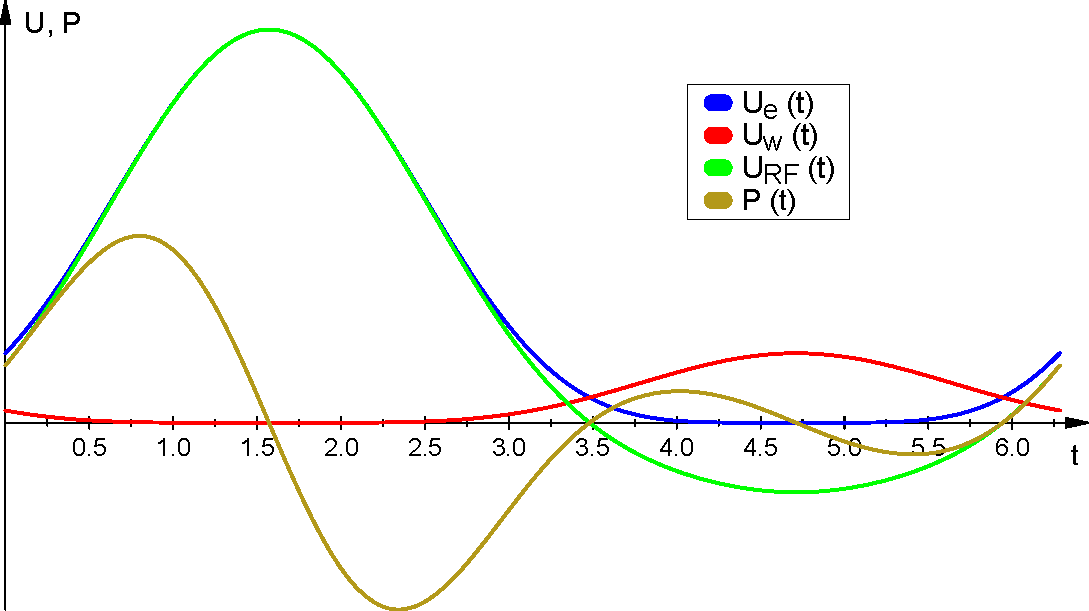
\includegraphics[width=0.75\columnwidth]{clipart/Bias-RF-voltage}
\par\end{centering}
\caption{\label{fig:Temporal-progression}Temporal progression of $U_{\mathrm{RF}}=U_{e}-U_{w}$,
$U_{e}$, $U_{e}$ and $P$ for $A_{w}/A_{e}=2$.}
\end{figure}

The power we have to input is
\begin{eqnarray}
P(t) & = & I_{\mathrm{RF}}\cos(\omega_{\mathrm{RF}}t)\cdot U_{\mathrm{RF}}(t)\label{eq:P-general}
\end{eqnarray}
In (\ref{eq:U_RF(t)}) we see that the term $\left(1-\sin(\omega_{\mathrm{RF}}t)\right)^{5/2}$
can be neglected for $\left(\cfrac{A_{w}}{A_{e}}\right)^{5/2}>50$
(error is then < 2\,\%). Using this in (\ref{eq:P-general}) gives
\begin{equation}
P(t)=I_{\mathrm{RF}}\cos(\omega_{\mathrm{RF}}t)\,\frac{2}{5n_{0}\epsilon_{0}^{3/2}}\,\left(\frac{I_{\mathrm{RF}}}{A_{w}\omega_{\mathrm{RF}}}\right)^{5/2}\sqrt{\frac{\lambda}{e\,k_{B}T_{e}}}\left(\frac{A_{w}}{A_{e}}\right)^{5/2}\left(1+\sin(\omega_{\mathrm{RF}}t)\right)^{5/2}
\end{equation}

The temporal progression of $P(t)$ is shown in \ref{fig:Temporal-progression}.
The generators measure the root mean square (RMS) of $P(t)$ as effective
power. The RMS of the term $\cos(\omega_{\mathrm{RF}}t)\cdot\left(1+\sin(\omega_{\mathrm{RF}}t)\right)^{5/2}$
is $\approx1.436$. We can therefore write
\begin{eqnarray}
P_{\mathrm{measured}} & = & I_{\mathrm{RF}}\,\frac{1.436\cdot2}{5n_{0}\epsilon_{0}^{3/2}}\,\left(\frac{I_{\mathrm{RF}}}{A_{w}\omega_{\mathrm{RF}}}\right)^{5/2}\sqrt{\frac{\lambda}{e\,k_{B}T_{e}}}\left(\frac{A_{w}}{A_{e}}\right)^{5/2}\nonumber \\
 & = & I_{\mathrm{RF}}^{7/2}\,\frac{1.436\cdot2}{5n_{0}\epsilon_{0}^{3/2}}\,\left(\frac{1}{A_{e}\omega_{\mathrm{RF}}}\right)^{5/2}\sqrt{\frac{\lambda}{e\,k_{B}T_{e}}}\\
I_{\mathrm{RF}} & = & \left(\frac{1.436\cdot2}{5P_{\mathrm{measured}}n_{0}\epsilon_{0}^{3/2}}\,\left(\frac{1}{A_{e}\omega_{\mathrm{RF}}}\right)^{5/2}\sqrt{\frac{\lambda}{e\,k_{B}T_{e}}}\right)^{-2/7}\nonumber \\
 & = & \left(\frac{5P_{\mathrm{measured}}n_{0}\epsilon_{0}^{3/2}}{1.436\cdot2}\right)^{2/7}\left(\frac{e\,k_{B}T_{e}}{\lambda}\right)^{1/7}\left(A_{e}\omega_{\mathrm{RF}}\right)^{5/7}
\end{eqnarray}

This could now be put into (\ref{eq:U_bias}):
\begin{eqnarray}
U_{\mathrm{bias}} & = & \frac{1.92\cdot2}{5n_{0}\epsilon_{0}^{3/2}}\,\left(\frac{\left(\frac{5P_{\mathrm{measured}}n_{0}\epsilon_{0}^{3/2}}{1.436\cdot2}\right)^{2/7}\left(\frac{e\,k_{B}T_{e}}{\lambda}\right)^{1/7}\left(A_{e}\omega_{\mathrm{RF}}\right)^{5/7}}{A_{w}\omega_{\mathrm{RF}}}\right)^{5/2}\sqrt{\frac{\lambda}{e\,k_{B}T_{e}}}\,\left(\frac{A_{w}}{A_{e}}\right)^{5/2}\nonumber \\
 & = & \frac{0.831}{n_{0}\epsilon_{0}^{3/2}\omega_{\mathrm{RF}}^{5/2}}\,\left(\left(P_{\mathrm{measured}}n_{0}\epsilon_{0}^{3/2}\right)^{2/7}\left(\frac{e\,k_{B}T_{e}}{\lambda}\right)^{1/7}\left(A_{e}\omega_{\mathrm{RF}}\right)^{5/7}\right)^{5/2}\sqrt{\frac{\lambda}{e\,k_{B}T_{e}}}\,\left(\frac{1}{A_{e}}\right)^{5/2}\nonumber \\
 & = & \frac{0.831}{n_{0}^{2/7}\epsilon_{0}^{3/7}}\,\left(\frac{P_{\mathrm{measured}}}{\omega_{\mathrm{RF}}A_{e}}\right)^{5/7}\left(\frac{\lambda}{e\,k_{B}T_{e}}\right)^{1/7}\label{eq:U-Bias-power}
\end{eqnarray}

and (\ref{eq:s_e-mean}) but this doesn't help us as long as we don't
know the electron temperature. We therefore go back to the matrix
model approximation.

\subsection{Approximation}

We already found (\ref{eq:U_sheath-approx-detail}):
\begin{equation}
U_{w\,\mathrm{matrix}}(t)=\frac{en_{0}}{2\epsilon_{0}}\left(\frac{I_{\mathrm{RF}}}{e\,n_{0}A_{w}\omega_{\mathrm{RF}}}\,\left(1-\sin(\omega_{\mathrm{RF}}t)\right)\right)^{2}
\end{equation}
and with (\ref{eq:U-matrix-relation}) we get
\begin{equation}
U_{\mathrm{RF}}(t)=\frac{en_{0}}{2\epsilon_{0}}\left(\frac{I_{\mathrm{RF}}}{e\,n_{0}A_{w}\omega_{\mathrm{RF}}}\right)^{2}\left(\left(\frac{A_{w}}{A_{e}}\right)^{2}\left(1+\sin(\omega_{\mathrm{RF}}t)\right)^{2}-\left(1-\sin(\omega_{\mathrm{RF}}t)\right)^{2}\right)
\end{equation}

To calculate the power we assume that $\left(\cfrac{A_{w}}{A_{e}}\right)^{2}\gg1$
so that we have to find only the RMS of the term $\cos(\omega_{\mathrm{RF}}t)\cdot\left(1+\sin(\omega_{\mathrm{RF}}t)\right)^{2}\raisebox{5mm}{}$.
This is $\approx1.146$ so that we can now write
\begin{eqnarray}
P_{\mathrm{measured}} & = & I_{\mathrm{RF}}\,\frac{1.146\cdot en_{0}}{2\epsilon_{0}}\left(\frac{I_{\mathrm{RF}}}{e\,n_{0}A_{w}\omega_{\mathrm{RF}}}\right)^{2}\left(\frac{A_{w}}{A_{e}}\right)^{2}\nonumber \\
 & = & I_{\mathrm{RF}}^{3}\,\frac{1.146}{2\epsilon_{0}en_{0}}\left(\frac{1}{A_{e}\omega_{\mathrm{RF}}}\right)^{2}\\
I_{\mathrm{RF}} & = & \left(A_{e}\,\omega_{\mathrm{RF}}\right)^{2/3}\,\left(\frac{2\epsilon_{0}en_{0}P_{\mathrm{measured}}}{1.146}\right)^{1/3}\label{eq:I_RF-approx}
\end{eqnarray}
Putting this relation for $I_{\mathrm{RF}}$ into (\ref{eq:U_w-matrix-mean})
gives
\begin{eqnarray}
U_{\mathrm{bias}} & = & \frac{1}{2e\epsilon_{0}n_{0}}\,\left(\frac{I_{\mathrm{RF}}}{A_{w}\,\omega_{\mathrm{RF}}}\right)^{2}\left(\frac{A_{w}}{A_{e}}\right)^{2}\\
 & = & \frac{1}{2e\epsilon_{0}n_{0}}\,\left(\frac{\left(A_{e}\,\omega_{\mathrm{RF}}\right)^{2/3}\,\left(\frac{2\epsilon_{0}en_{0}P_{\mathrm{measured}}}{1.146}\right)^{1/3}}{A_{e}\,\omega_{\mathrm{RF}}}\right)^{2}\left(\frac{A_{w}}{A_{e}}\right)^{2}\nonumber \\
 & = & \left(\frac{1}{2e\epsilon_{0}n_{0}}\right)^{1/3}\,\left(\frac{P_{\mathrm{measured}}}{1.146\cdot A_{e}\,\omega_{\mathrm{RF}}}\right)^{2/3}\left(\frac{A_{w}}{A_{e}}\right)^{2}
\end{eqnarray}
and this can be transformed to deliver the plasma density:
\begin{eqnarray}
n_{0}^{1/3} & = & \frac{1}{U_{\mathrm{bias}}}\,\left(\frac{1}{2e\epsilon_{0}}\right)^{1/3}\,\left(\frac{P_{\mathrm{measured}}}{1.146\cdot A_{e}\,\omega_{\mathrm{RF}}}\right)^{2/3}\left(\frac{A_{w}}{A_{e}}\right)^{2}\nonumber \\
n_{0} & = & \frac{1}{2e\epsilon_{0}U_{\mathrm{bias}}^{3}}\,\left(\frac{P_{\mathrm{measured}}}{1.146\cdot A_{e}\,\omega_{\mathrm{RF}}}\right)^{2}\left(\frac{A_{w}}{A_{e}}\right)^{6}\label{eq:n_0-approx}
\end{eqnarray}

With this approximated plasma density we can also approximate the
ionization ratio $\Gamma_{i}$:
\begin{equation}
\Gamma_{i}=\frac{N}{Vn_{0}}=\frac{p}{k_{B}T\,n_{0}}\label{eq:ionization-ratio}
\end{equation}
where $N$ is the number of particles in the plasma chamber, $p$
is the pressure, $V$ the volume of the chamber and $T$ the global
temperature in the chamber.

Although (\ref{eq:n_0-approx}) is an approximation, we can put it
into the precise relation (\ref{eq:U_w-precise}) to get a feeling
how the electron temperature behaves:
\begin{eqnarray}
U_{\mathrm{bias}} & = & \frac{1.92\cdot2}{5n_{0}\epsilon_{0}^{3/2}}\,\left(\frac{I_{\mathrm{RF}}}{A_{w}\omega_{\mathrm{RF}}}\right)^{5/2}\,\left(\frac{ek_{B}T_{e}}{\lambda}\right)^{-1/2}\left(\frac{A_{w}}{A_{e}}\right)^{5/2}\nonumber \\
\frac{ek_{B}T_{e}}{\lambda} & = & \left(\frac{1.92\cdot2}{5n_{0}\epsilon_{0}^{3/2}U_{\mathrm{bias}}}\,\left(\frac{I_{\mathrm{RF}}}{A_{w}\omega_{\mathrm{RF}}}\right)^{5/2}\,\left(\frac{A_{w}}{A_{e}}\right)^{5/2}\right)^{2}\nonumber \\
T_{e} & = & \left(\frac{1.92\cdot2}{5}\right)^{2}\left(\frac{I_{\mathrm{RF}}}{A_{e}\,\omega_{\mathrm{RF}}}\right)^{5}\frac{\lambda}{n_{0}^{2}\,\epsilon_{0}^{3}\,U_{\mathrm{bias}}^{2}\,ek_{B}}\label{eq:T_e-wrong}\\
 & = & \left(\frac{1.92\cdot2}{5}\right)^{2}\left(\frac{\left(\frac{5P_{\mathrm{measured}}n_{0}\epsilon_{0}^{3/2}}{1.436\cdot2}\right)^{2/7}\left(\frac{e\,k_{B}T_{e}}{\lambda}\right)^{1/7}\left(A_{e}\omega_{\mathrm{RF}}\right)^{5/7}}{A_{e}\,\omega_{\mathrm{RF}}}\right)^{5}\frac{\lambda}{n_{0}^{2}\,\epsilon_{0}^{3}\,U_{\mathrm{bias}}^{2}\,ek_{B}}\nonumber \\
 & = & \left(\left(\frac{1.92\cdot2}{5}\right)^{2}\left(\frac{5P_{\mathrm{measured}}n_{0}\epsilon_{0}^{3/2}}{1.436\cdot2}\right)^{10/7}\left(\frac{e\,k_{B}}{\lambda}\right)^{5/7}\frac{1}{\left(A_{e}\omega_{\mathrm{RF}}\right)^{10/7}}\,\frac{\lambda}{n_{0}^{2}\,\epsilon_{0}^{3}\,U_{\mathrm{bias}}^{2}\,ek_{B}}\right)^{7/2}\nonumber \\
 & = & \left(\frac{1.92\cdot2}{5}\right)^{7}\left(\frac{5P_{\mathrm{measured}}}{1.436\cdot2}\right)^{5}\frac{\lambda}{n_{0}^{2}ek_{B}\,\left(A_{e}\omega_{\mathrm{RF}}\right)^{5}\epsilon_{0}^{3}\,U_{\mathrm{bias}}^{7}}
\end{eqnarray}


\subsection{Conclusions}

\begin{figure}[h]
\begin{centering}
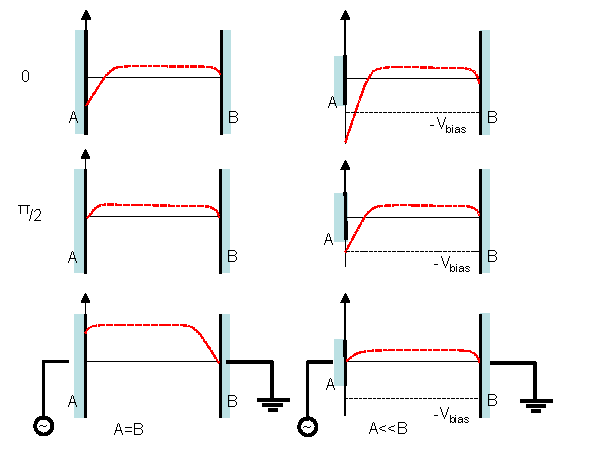
\includegraphics[width=0.75\columnwidth]{clipart/Bias-Geometry}
\par\end{centering}
\caption{\label{fig:Spatial-progression}Spatial progression of the voltage
in a plasma between symmetric and asymmetric electrode areas. Image
from \cite{Keudell12}.}
\end{figure}

\ref{fig:Spatial-progression} shows the spatial progression of the
voltage inside a plasma schematically. Due to the smaller electrode
area the voltage across the sheath above the electrode is much higher.
This is the effect we use to accelerate ions towards substrates to
coat them. (\ref{eq:U_bias}) shows that a smaller $A_{e}$ leads
to less necessary input current (and thus input power) to get the
same bias voltage.

Interesting is the inverse cubic dependence of the bias voltage in
(\ref{eq:n_0-approx}). So a low plasma density results in a high
bias. This is an important result because this is the reason why a
dense plasma is burning into holes of substrates at the electrode
for low ionized plasmas. These are typically plasmas of mainly larger
precursor molecules. This topic is discussed in detail in \ref{sec:Hollow-cathode-effect}.

\begin{figure}[h]
\begin{centering}
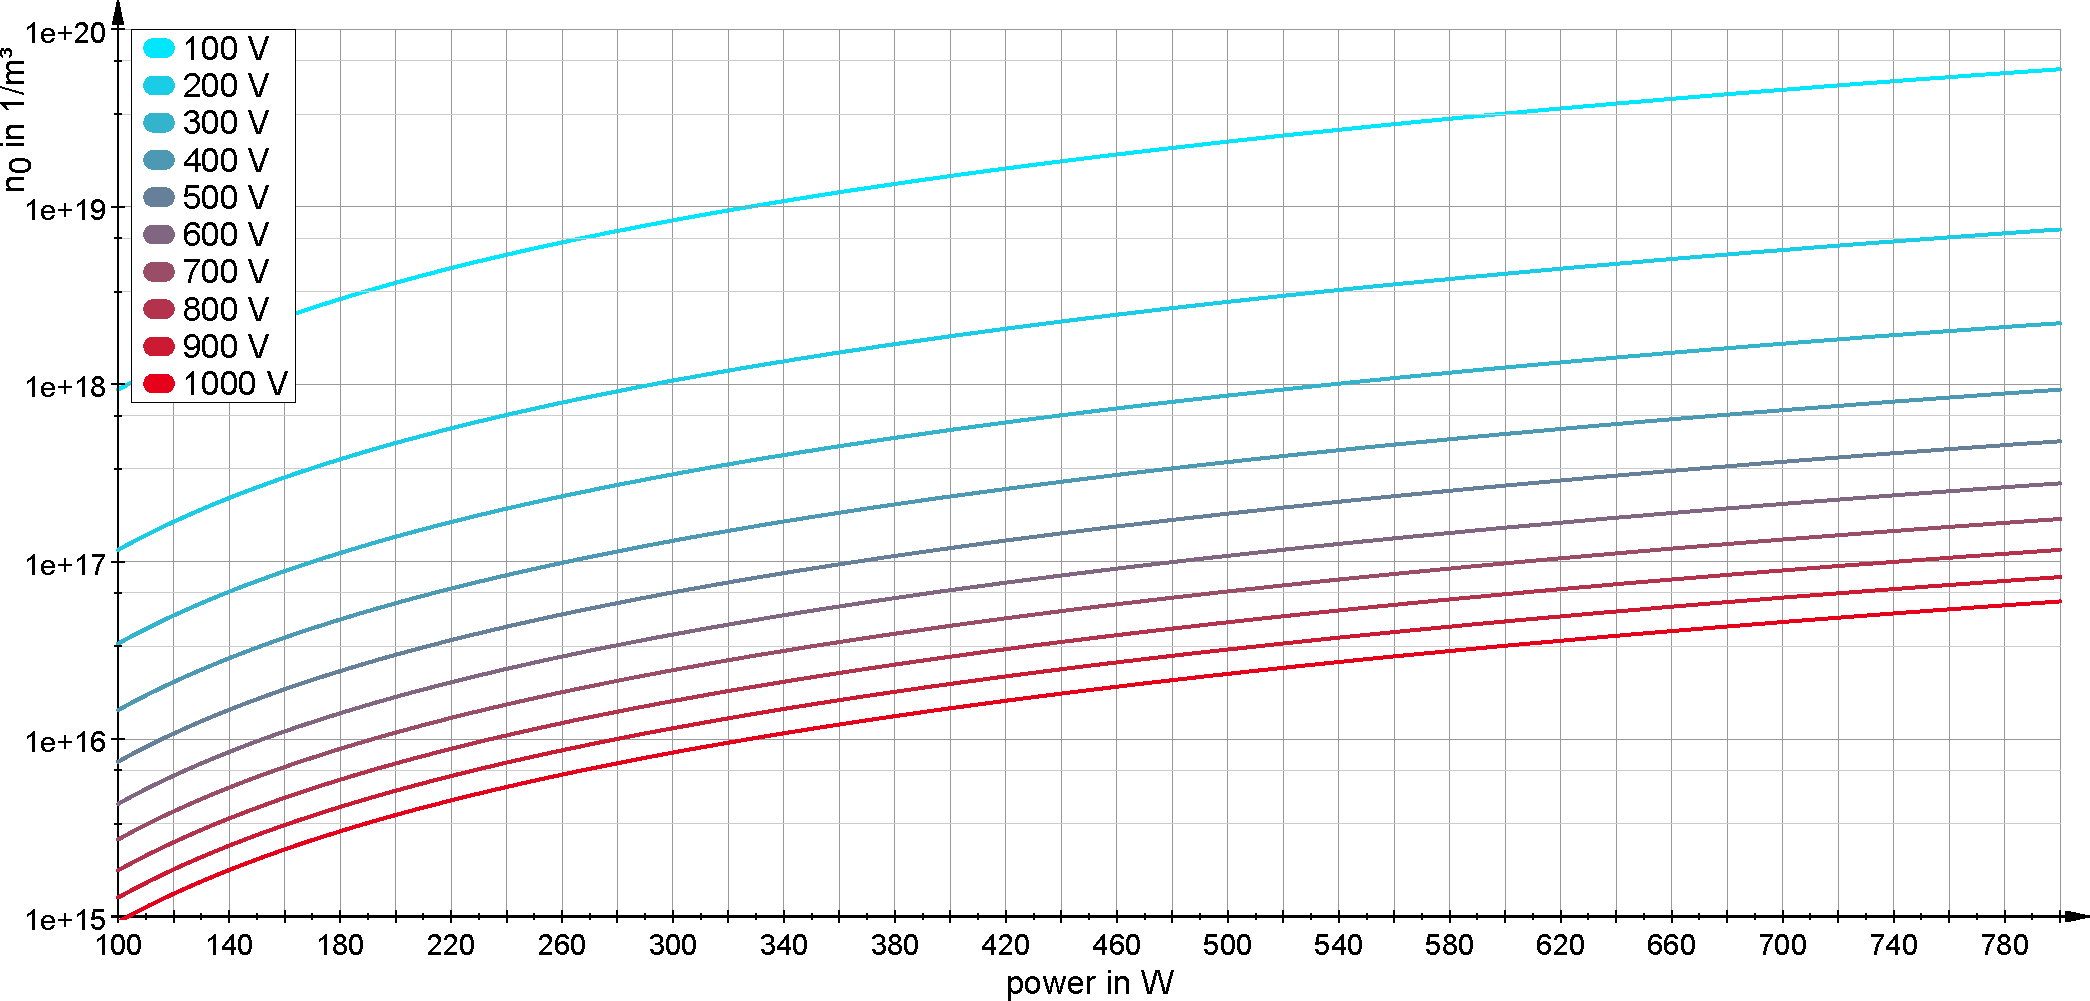
\includegraphics[width=1\columnwidth]{clipart/plasma-density-Domino}
\par\end{centering}
\caption{\label{fig:Plasma-density-Domino}Plasma density for the plasma device
``Domino'' with a chamber volume of 80\,l ($A_{e}\approx0.138\,$m\texttwosuperior ,
$A_{w}\approx0.832$\,m\texttwosuperior ) in dependence of the applied
plasma power and the measured $U_{\mathrm{bias}}$.}
\end{figure}

\begin{figure}[!h]
\begin{centering}
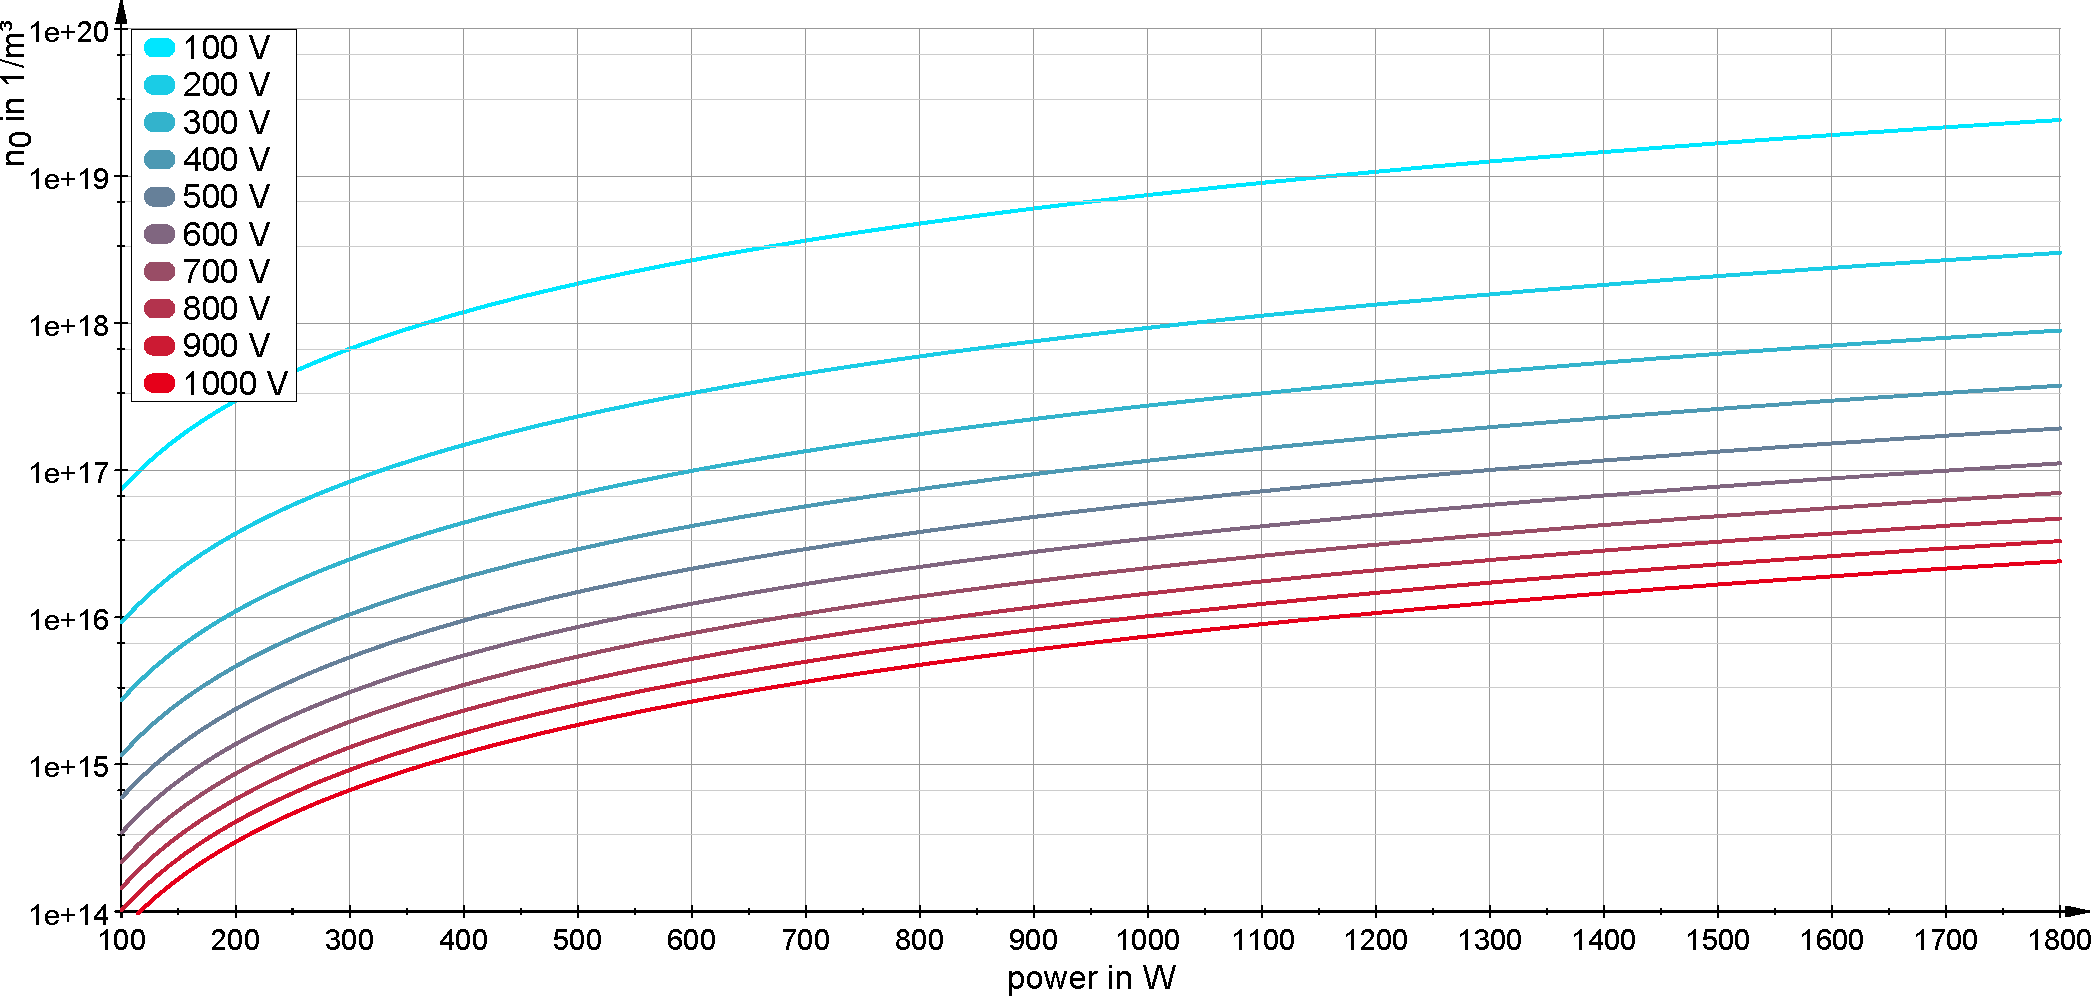
\includegraphics[width=1\columnwidth]{clipart/plasma-density-Porta900}
\par\end{centering}
\caption{\label{fig:Plasma-density-Porta}Plasma density for the plasma device
``Porta~900'' with one large electrode ($A_{e}=0.64\,$m\texttwosuperior ,
$A_{w}=0.9^{2}\cdot6-0.64=4.22$\,m\texttwosuperior ) in dependence
of the applied plasma power and the measured $U_{\mathrm{bias}}$.
For the setup with 3~chambers ($A_{e}=0.07\,$m\texttwosuperior ,
$A_{w}=2.594$\,m\texttwosuperior ) the values in this plot must
be multiplied with the factor 198.16.}
\end{figure}

The plasma density $n_{0}$ for the 80\,l chamber device ``Domino''\footnote{Manufacturer: Plasma Electronic; device details: \href{https://www.plasma-electronics.com/domino.html}{https://www.plasma-electronics.com/domino.html}}
is shown in \ref{fig:Plasma-density-Domino}, the plasma density for
a 720\,l chamber device ``Porta~900''\footnote{Manufacturer: Plasma Electronic; cubic chamber with an edge length
of 0.9\,m;\\
device details: \href{https://www.plasma-electronics.com/porta.html}{https://www.plasma-electronics.com/porta.html}} in \ref{fig:Plasma-density-Porta}. One can see that if one measures
for a low power a relatively high bias, the plasma density is low
meaning the ionization rate is also low. By modifying the ``Porta~900''
so that the device chamber is divided by 3~equally sized inner chambers
with each a smaller electrode, the plasma density is increased by
about a factor~200. So the then different ratio $A_{e}/A_{w}$ change
the plasma parameters drastically.

Taking the case that in the ``Domino'' we measured a bias of 500\,V
for pure Ar at $p=2\,$Pa with a power of 190\,W. With \ref{fig:Plasma-density-Domino}
we get $n_{0}\approx1.5\cdot10^{14}\,$1/m\textthreesuperior{} and
therefore with (\ref{eq:T_e-wrong}) $T_{e}\approx7.6\cdot10^{5}\,$K.
But this about 100~times higher than values found in literature and
with (\ref{eq:Phi_float}) we would get a plasma potential of about
327\,V. This shows that the electron temperature cannot be estimated
using the matrix model in its derivation. This result could have been
expected because the matrix model does not take care of $T_{e}$.
In fact one cannot estimate $T_{e}$ by measuring only the plasma
power and the bias voltage.

\subsection{Applications}

\subsubsection{ICP + CCP}

Looking at (\ref{eq:U-Bias-power}):
\begin{equation}
U_{\mathrm{bias}}=\frac{0.831}{n_{0}^{2/7}\epsilon_{0}^{3/7}}\,\left(\frac{P_{\mathrm{measured}}}{\omega_{\mathrm{RF}}A_{e}}\right)^{5/7}\left(\frac{\lambda}{e\,k_{B}T_{e}}\right)^{1/7}
\end{equation}
 we see that $U_{\mathrm{bias}}\sim n_{0}^{-2/7}$, $U_{\mathrm{bias}}\sim P_{\mathrm{measured}}^{5/7}$
and $U_{\mathrm{bias}}\sim T_{e}^{-1/7}$. For a setup where the ions
are generated in an \href{https://en.wikipedia.org/wiki/Inductively_coupled_plasma}{inductively coupled plasma}
(ICP), the ion energy is a constant while the ion density increases
with increasing input power for the ICP. To get a defined and adjustable
ion impact energy on the substrate one can apply an RF-voltage to
the substrate. We then have a \href{https://en.wikipedia.org/wiki/Capacitively_coupled_plasma}{capacitively coupled plasma}
(CCP) above the substrate but $n_{0}$ is almost independent of the
CCP parameters.

For a glass etching application this setup was chosen. For the ICP
and the CCP the same frequency was used. As both plasmas did not interfere
in this setup although the same frequency was used, they can be treated
as being independent from each other. Then for a constant ICP power
and thus a constant $n_{0}$ the bias voltage should have the dependency
$U_{\mathrm{bias}}\sim P_{\mathrm{measured}}^{5/7}$ for the case
that the CCP does not change the electron temperature $T_{e}$. The
measurements to prove this theory was performed using an ICP source
model ``Copra DN 160''\footnote{Manufacturer: CCR technology;\\
device details: \href{https://www.ccrtechnology.de/copra-products/copra-round-sources/}{https://www.ccrtechnology.de/copra-products/copra-round-sources/}}. The result is plotted in \ref{fig:Dependency-Bias-ICP}. Fitting
the curves in this plot with the function $U_{\mathrm{bias}}=K\cdot P_{\mathrm{measured}}^{X}$
gives the results listed in \ref{tab:Fit-parameters}. The expected
exponent $5/7\approx0.71$ is the one for 300\,W. For larger ICP
powers the exponent increases which implies that $T_{e}$ is then
smaller.

\begin{figure}[h]
\begin{centering}
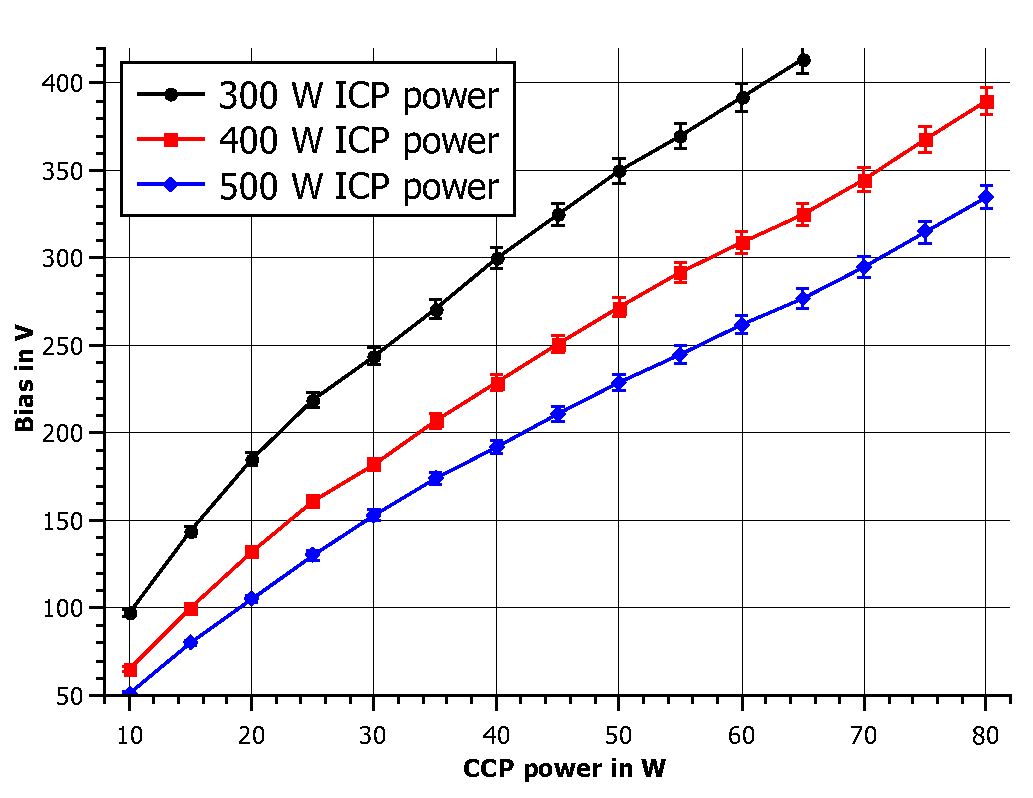
\includegraphics[width=0.7\columnwidth]{clipart/ICP-CCP-Bias}
\par\end{centering}
\caption{\label{fig:Dependency-Bias-ICP}Dependency of the bias voltage on
the CCP power for different ICP powers.}
\end{figure}

\begin{table}[h]
\caption{\label{tab:Fit-parameters}Fit parameters for the measurement curves
from \ref{fig:Dependency-Bias-ICP}.}

\centering{}%
\begin{tabular}{|c|c|c|c|}
\hline 
ICP power in W & Parameter $X$ & Parameter $K$ & $\chi_{\mathrm{red}}^{2}$ of the fit\tabularnewline
\hline 
\hline 
300 & $0.71\pm0.01$ & $73.71\pm9.09$ & 1.12\tabularnewline
\hline 
400 & $0.79\pm0.01$ & $22.82\pm2.06$ & 1.58\tabularnewline
\hline 
500 & $0.82\pm0.01$ & $14.82\pm1.16$ & 1.31\tabularnewline
\hline 
\end{tabular}
\end{table}

The ion current density in the used ICP source for a fixed pressure
of 0.1\,Pa is for an input power of 300\,W about 0.1\,mA/cm\texttwosuperior{}
and for 500\,W about 0.21\,mA/cm\texttwosuperior . Although we measured
at a pressure of about 0.4\,Pa we assume that also $n_{0}$ is increased
by a factor 1.75 if going from 300 to 500\,W ICP power. For low CCP
powers we can neglect the influence of the CCP on $n_{0}$ and expect
that the bias voltage for 500\,W is $1.75^{2/7}\approx0.44$ lower
than for 300\,W. Looking at \ref{fig:Dependency-Bias-ICP} we get
a factor 0.53 -- 0.67 lower bias voltage, depending on the CCP power,
see \ref{tab:Factors-of-the}. Even for the lowest measurable CCP
power of 10\,W we see again that an increasing ICP power decreases
$T_{e}$ as the factor is much greater than expected. For higher CCP
powers we have also a lower $T_{e}$. This is an interesting result
because a higher CCP power always leads to a higher $n_{0}$ and this
decreases the bias.

\begin{table}[h]
\caption{\label{tab:Factors-of-the}Factors of the decreasing bias voltages
when going from 300 to 500\,W ICP power; in dependence of the CCP
power.}

\centering{}%
\begin{tabular}{|c|c|c|c|c|c|c|c|}
\hline 
CCP power in W & 10 & 15 & 20 & 30 & 40 & 50 & 60\tabularnewline
\hline 
\hline 
Factor & 0.53 & 0.55 & 0.56 & 0.62 & 0.64 & 0.65 & 0.67\tabularnewline
\hline 
\end{tabular}
\end{table}


\subsubsection{CCP}

In contrary to the combination of ICP~+~CCP, for a pure CCP the
Bias voltage behave differently. According to (\ref{eq:U-Bias-power}):
\begin{equation}
U_{\mathrm{bias}}=\frac{0.831}{n_{0}^{2/7}\epsilon_{0}^{3/7}}\,\left(\frac{P_{\mathrm{measured}}}{\omega_{\mathrm{RF}}A_{e}}\right)^{5/7}\left(\frac{\lambda}{e\,k_{B}T_{e}}\right)^{1/7}
\end{equation}
 one gets the relations $U_{\mathrm{bias}}\sim n_{0}^{-2/7}$ and
$U_{\mathrm{bias}}\sim P_{\mathrm{measured}}^{5/7}$. In a CCP an
increased $P$ will also always result in an increased $n_{0}$ and
a changed $T_{e}$. For practical applications it is helpful to know
how the Bias is changed by changing the input power and the pressure
$p$.

For the measurement the device ``Labor~1'' (80~liter vacuum chamber)
was used. Pure argon was used as process gas because it is a single-atom
gas (to keep the pressure constant because no molecule fragmentation
can occur). The Bias voltage was measured at constant pressures while
the input power was changed. The resulting datasets were fit using
these equations
\begin{equation}
U_{\mathrm{bias}}=K\cdot\left(P_{\mathrm{measured}}-x_{0}\right)^{B_{\mathrm{powerr}}}+y_{0}
\end{equation}
\begin{equation}
U_{\mathrm{bias}}=K\cdot\left(p-x_{0}\right)^{B_{\mathrm{pressure}}}+y_{0}
\end{equation}

\ref{fig:Dependency-Bias-CCP} shows as example how the results looked.
It can be seen that the fit at constant pressure well describes the
change of the Bias whereas the fit at constant pressure shows that
the fit model is not optimal ($\chi_{\mathrm{red}}>1$). In \ref{fig:Dependency-Bias-CCP-final}
the fit parameters $B_{\mathrm{power}}$ and $B_{\mathrm{pressure}}$
are plotted for the different pressures and powers, receptively. One
can see that the fit parameters are relatively constant for the different
pressures and powers. As final conclusion one gets for a CCP with
argon:
\begin{equation}
U_{\mathrm{bias}}\sim P_{\mathrm{measured}}^{{\textstyle 0.5360\pm0.0152}}\label{eq:U-P-exponent}
\end{equation}
\begin{equation}
U_{\mathrm{bias}}\sim p^{{\textstyle -0.1831\pm0.0016}}\label{eq:U-p-exponent}
\end{equation}

This shows that the plasma density $n_{0}$ is indeed increased if
the pressure is increased. The electron temperature $T_{e}$ is increased
too so that the exponent in (\ref{eq:U-p-exponent}) is greater than
$-2/7$. If the CCP-power is increased $n_{0}$ and $T_{e}$ are increased
too so that the exponent in (\ref{eq:U-P-exponent}) is smaller than
$5/7$.

\begin{figure}[p]
\begin{centering}
\subfloat[Dependency of the bias voltage on the input power for a fixed pressure
of 4.14\,Pa.]{\begin{centering}
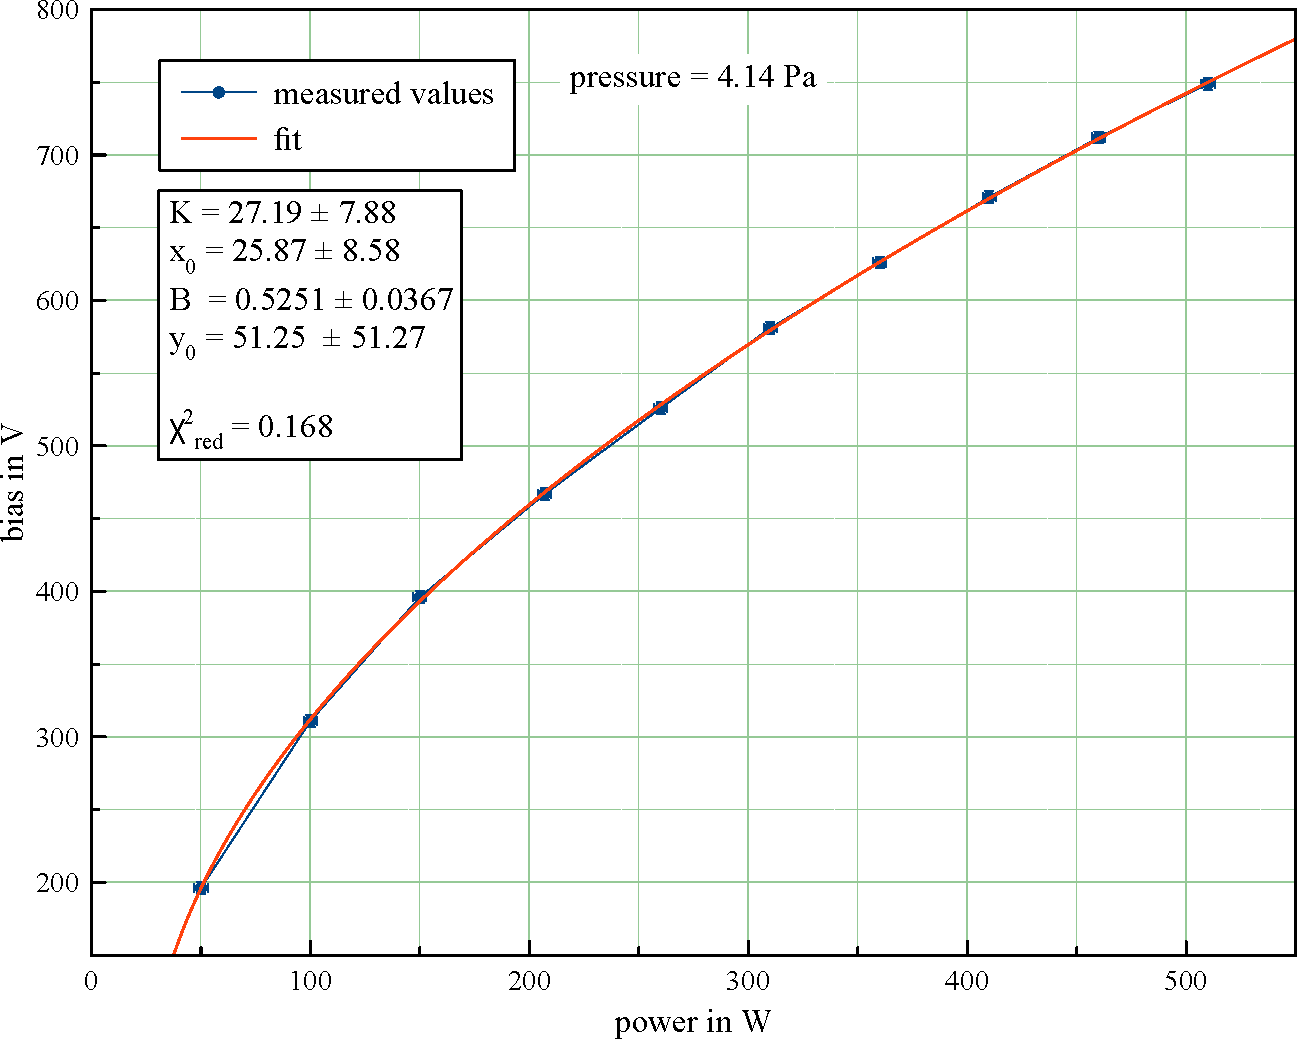
\includegraphics[width=0.8\columnwidth]{clipart/Power-Bias-at-4-14Pa}
\par\end{centering}
}
\par\end{centering}
\begin{centering}
\subfloat[Dependency of the bias voltage on the pressure for a fixed input power
of 400\,W.]{\begin{centering}
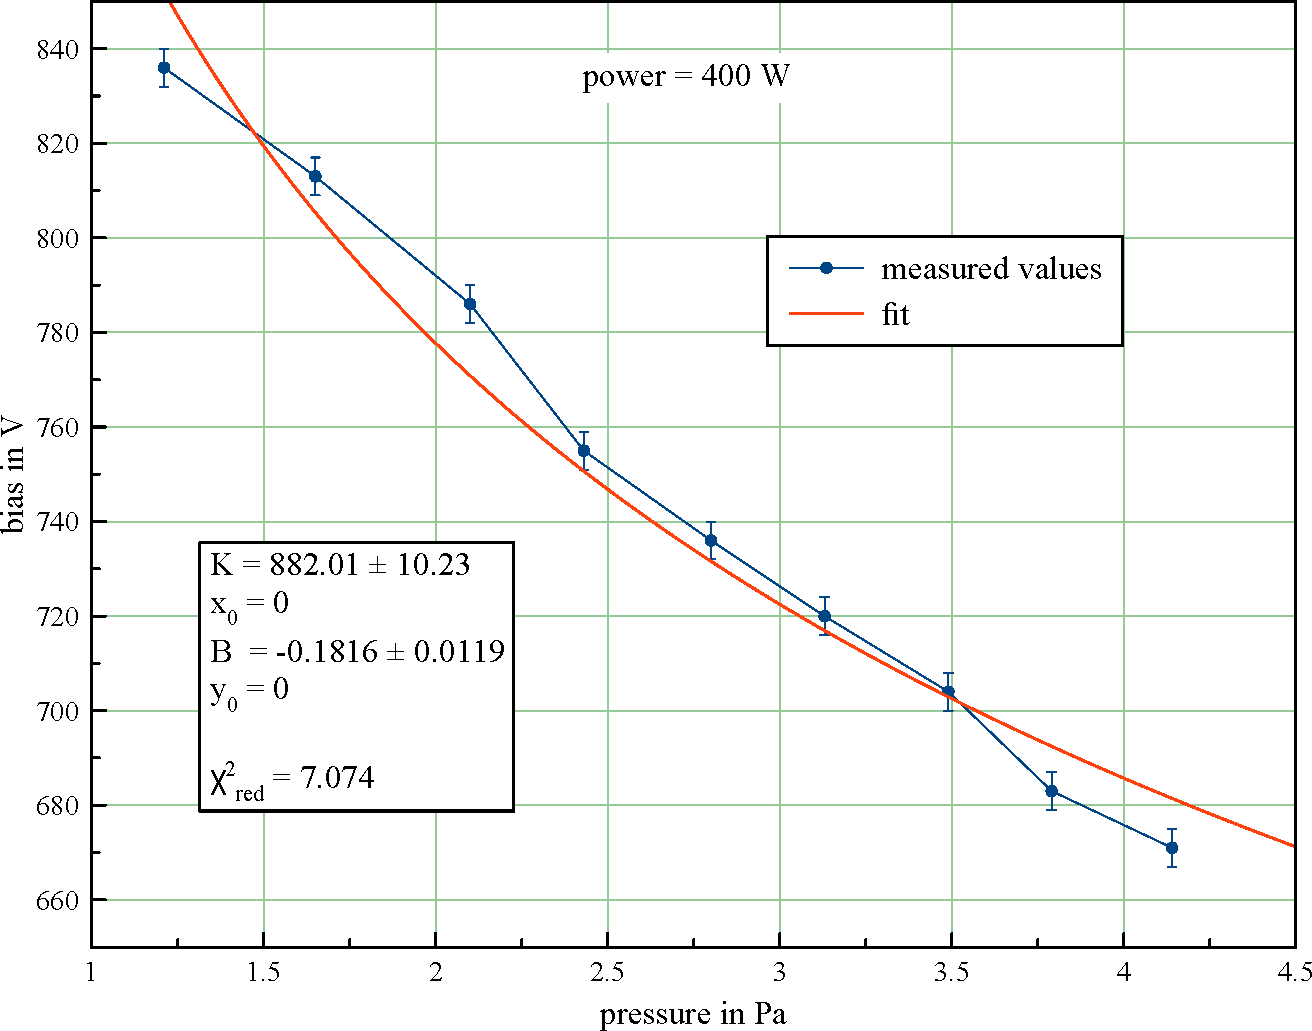
\includegraphics[width=0.8\columnwidth]{clipart/Pressure-Bias-at-400W}
\par\end{centering}
}
\par\end{centering}
\caption{\label{fig:Dependency-Bias-CCP}Dependency of the bias voltage on
the pressure and the input power for 2~different cases.}
\end{figure}

\begin{figure}[p]
\begin{centering}
\subfloat[Fit of the fit-parameters $B_{\mathrm{power}}$ at different pressures.]{\begin{centering}
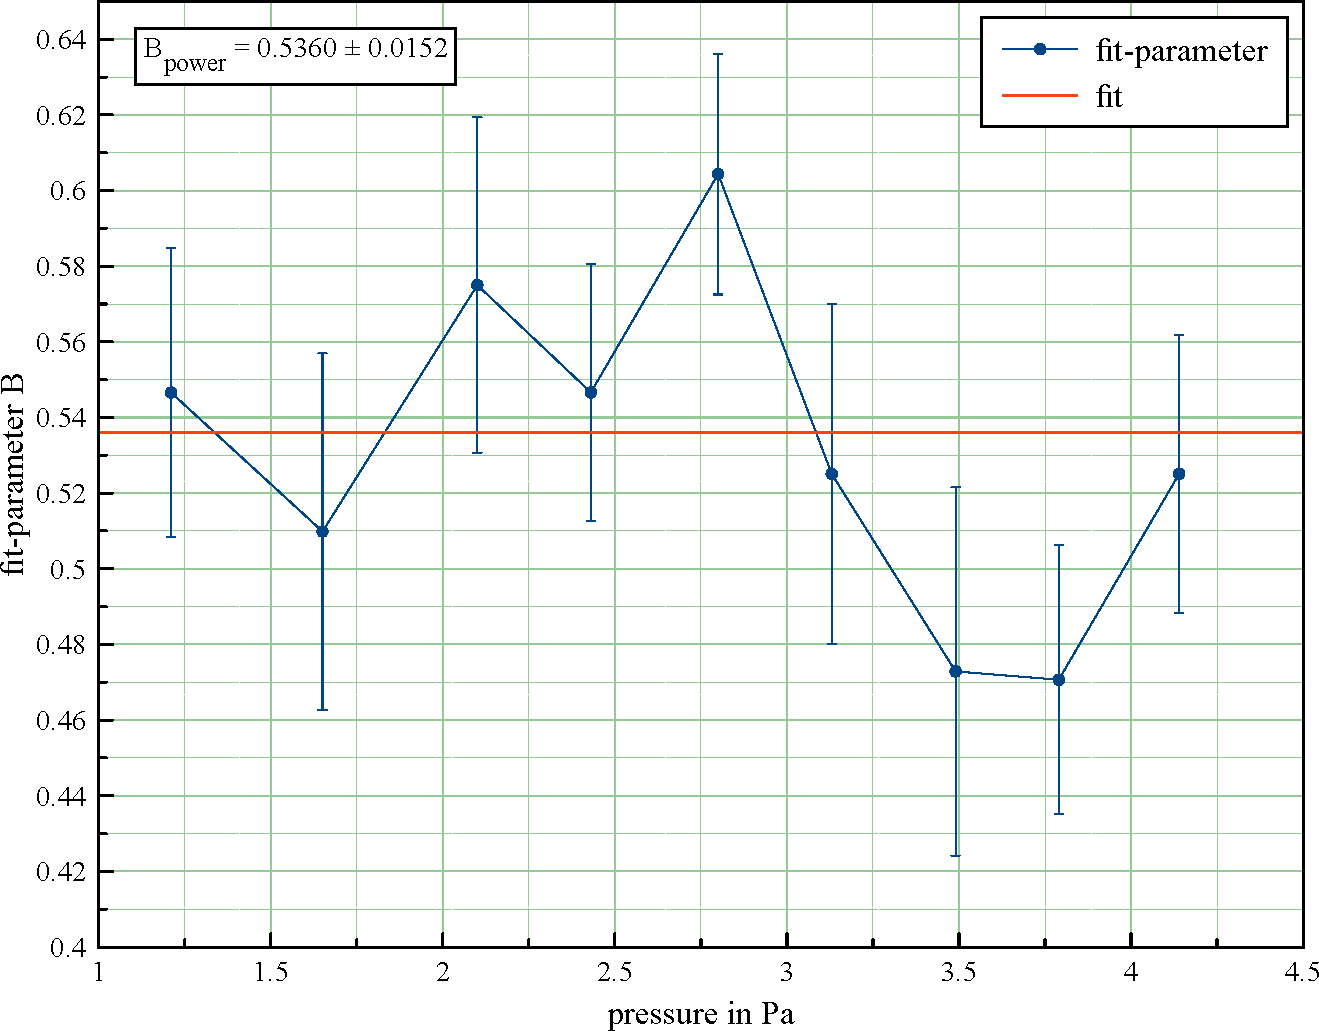
\includegraphics[width=0.85\columnwidth]{clipart/Bias-Exponent-Pressure}
\par\end{centering}
}
\par\end{centering}
\begin{centering}
\subfloat[Fit of the fit-parameters $B_{\mathrm{pressure}}$ at different input
powers.]{\begin{centering}
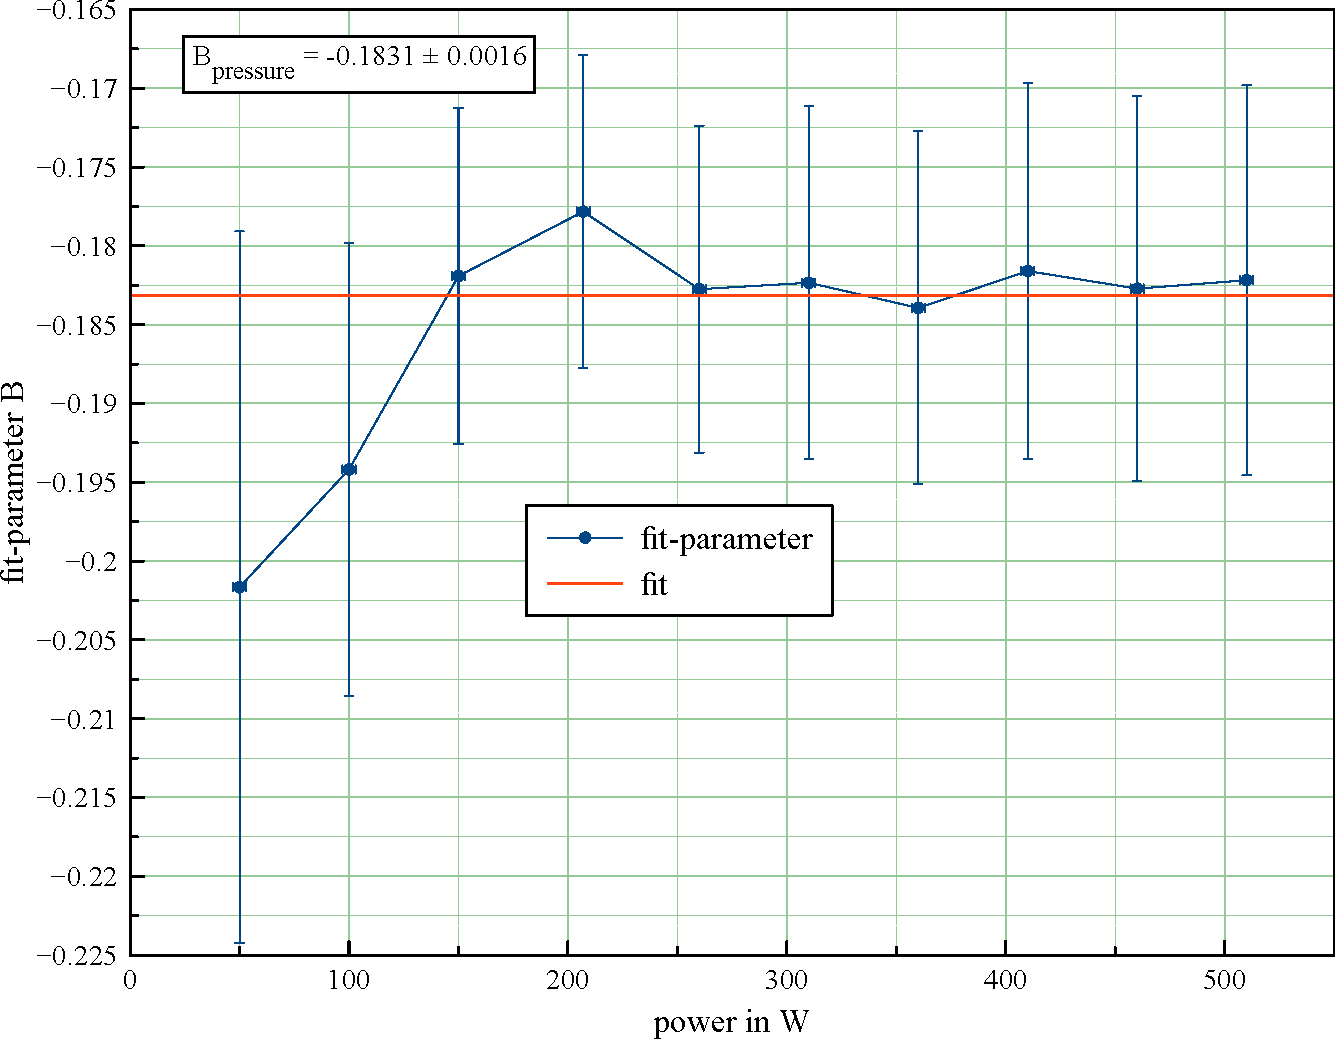
\includegraphics[width=0.85\columnwidth]{clipart/Bias-Exponent-Power}
\par\end{centering}
}
\par\end{centering}
\caption{\label{fig:Dependency-Bias-CCP-final}Linear fit of the different
fit-parameters $B_{\mathrm{power}}$ and $B_{\mathrm{pressure}}$.}
\end{figure}

\newpage{}

\section{Floating Potential}

When treating polymer substrates they are often placed into the chamber
without an electrical connection to the chamber walls or the electrode.
At the substrate there is therefore no sheath. The question is now
how large the potential between the plasma and the substrate will
be.

As there is no electric connection, the substrate is on a so-called
floating potential and the ion current $I_{i}$ must be equal the
electron current $I_{e}$ onto the substrate surface. So we can write
\begin{eqnarray}
I_{e} & = & I_{i}\nonumber \\
A\,n_{0}v_{e,\,\mathrm{therm}} & = & A\,n_{0}v_{B}\label{eq:charge-conservation}
\end{eqnarray}
where we used that the ions within the plasma must have the \noun{Bohm}
velocity.

Within the plasma we can assume that the electrical field is independent
of the position. Therefore the velocity of the electrons is their
thermal one $v_{e,\,\mathrm{therm}}$.

The mean $v_{e,\,\mathrm{therm}}$ can be calculated using the Maxwell-Boltzmann
distribution $f(v)$:
\begin{eqnarray}
\left\langle v_{e,\,\mathrm{therm}}\right\rangle  & = & \int vf(v)\,\mathrm{d}v\nonumber \\
 & = & \int v_{e}\,\sqrt{\frac{m_{e}}{2\pi k_{B}T_{e}}}\exp\left(\frac{-m_{e}v_{_{e}}^{2}}{2k_{B}T_{e}}\right)\,\mathrm{d}v_{e}\nonumber \\
 & = & -\sqrt{\frac{k_{B}T_{e}}{2\pi m_{e}}}\exp\left(\frac{-e\,\varPhi}{k_{B}T_{e}}\right)\label{eq:<e-therm>}
\end{eqnarray}
Where the relation $\cfrac{m_{e}v_{e}^{2}}{2}=e\,\varPhi$ was used.

(\ref{eq:charge-conservation}) becomes now 
\begin{eqnarray}
\sqrt{\frac{k_{B}T_{e}}{M}} & = & -\sqrt{\frac{k_{B}T_{e}}{2\pi m_{e}}}\exp\left(\frac{-e\,\varPhi_{\mathrm{float}}}{k_{B}T_{e}}\right)\nonumber \\
\varPhi_{\mathrm{float}} & = & \frac{k_{B}T_{e}}{e}\ln\left(\sqrt{\frac{2\pi m_{e}}{M}}\right)
\end{eqnarray}

In our devices the electrode is set to a certain voltage to apply
power to the plasma. Therefore we get a bias which is negative. Electrons
are therefore reflected and cannot reach the electrode surface (except
of one point in time). We therefore have instead of (\ref{eq:charge-conservation})
\begin{eqnarray}
A_{w}\,n_{0}v_{e,\,\mathrm{therm}} & = & n_{0}v_{B}\,(A_{w}+A_{e})
\end{eqnarray}
which leads to

\begin{eqnarray}
\sqrt{\frac{k_{B}T_{e}}{M}}\,(A_{w}+A_{e}) & = & -\sqrt{\frac{k_{B}T_{e}}{2\pi m_{e}}}\exp\left(\frac{-e\,\varPhi_{\mathrm{float}}}{k_{B}T_{e}}\right)A_{w}\nonumber \\
\varPhi_{\mathrm{float}} & = & \frac{k_{B}T_{e}}{e}\ln\left(\frac{A_{w}+A_{e}}{A_{w}}\,\sqrt{\frac{2\pi m_{e}}{M}}\right)\label{eq:Phi_float}
\end{eqnarray}

The influence of the ion mass $M=N\,$u ($\mathrm{u}=1.66\cdot10^{-27}\,$kg
is the atomic mass unit) on $\varPhi_{\mathrm{float}}$ is shown in
\ref{fig:floating-potential}. $\ce{O2}$ has a mass of 32\,u while
a large molecule like \href{https://en.wikipedia.org/wiki/Hexamethyldisiloxane}{HMDSO}
has a mass of 162~u. It can be seen that the potential does not increase
a lot with higher ion masses and for large molecules one has to have
in mind that they are cracked into smaller ones in the plasma so that
the real floating potential will not be far above the one of oxygen.

\begin{figure}[h]
\begin{centering}
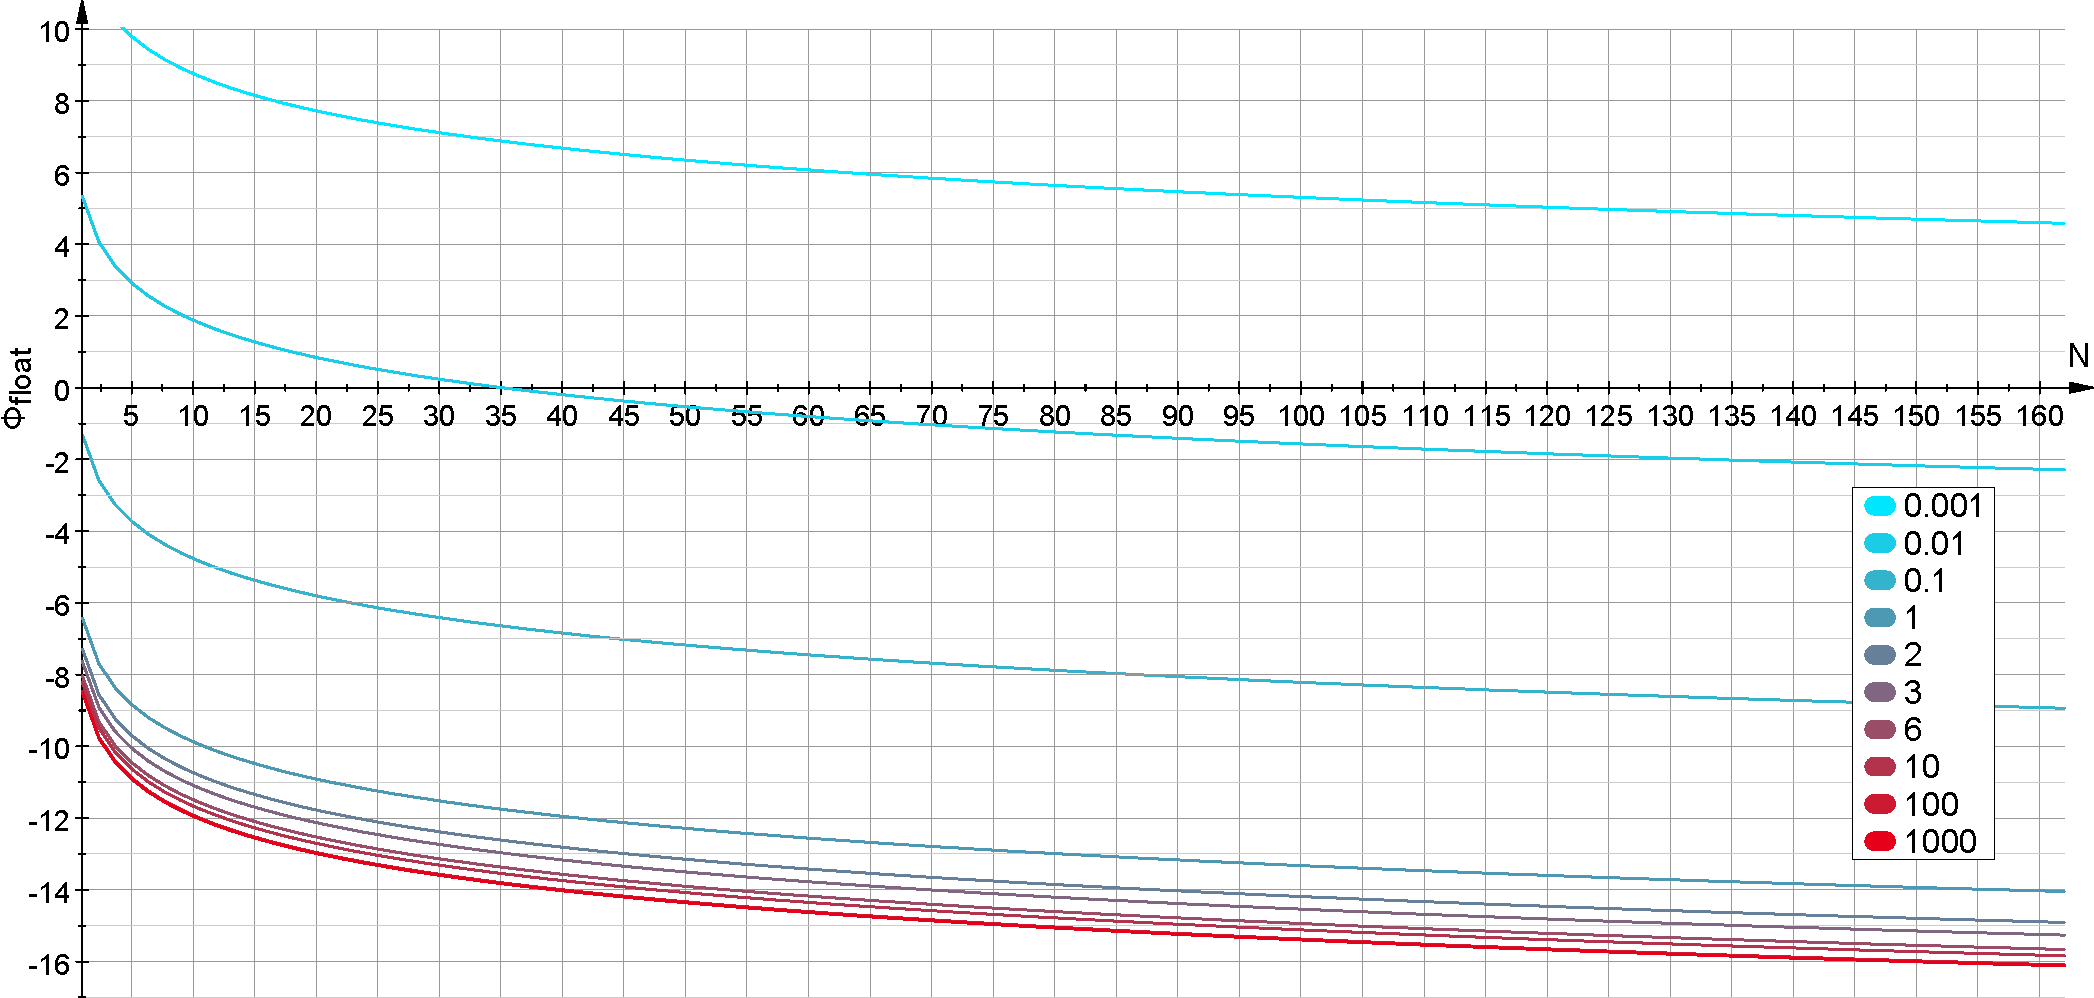
\includegraphics[width=1\columnwidth]{clipart/Floating-potential}
\par\end{centering}
\caption{\label{fig:floating-potential}$\Phi_{\mathrm{float}}$ in V in dependence
of the ion mass $M=N\,$u for different fractions $\cfrac{A_{w}}{A_{e}}$.
The electron temperature was set in the calculation to $T_{e}=3.48\cdot10^{4}\,$K.}
\end{figure}

As the ions must have the Bohm velocity, the potential to accelerate
the ions to the velocity is the plasma potential:
\begin{eqnarray}
e\,\varPhi_{\mathrm{plasma}} & = & \frac{Mv_{B}^{^{2}}}{2}\nonumber \\
\varPhi_{\mathrm{plasma}} & = & \frac{k_{B}T_{e}}{2e}
\end{eqnarray}

For a typical electron temperature of $T_{e}=3.48\cdot10^{4}\,$K
we have $\varPhi_{\mathrm{plasma}}\approx1.5\,$V.

\subsection*{Conclusion}

The floating potential is often greater than the voltage across the
sheath of a grounded chamber wall. Assuming we have a setup with $A_{w}=6A_{e}$
and measure $U_{\mathrm{bias}}=400\,$V we can calculate with (\ref{eq:U_bias-general})
that $U_{w}\approx4.5\,$V. If the electrode area is much larger than
the chamber wall area the plasma potential can be positive.

By measuring the floating potential with e.\,g.\ a \noun{Langmuir}
probe, we could measure the electron temperature and could then calculate
plasma potential, the real sheath thickness $s$ according to (\ref{eq:s_precise})
and also the real plasma density $n_{0}$ according to (\ref{eq:U_w-precise}).

\section{Dissipated Power}

The power in a CCP is dissipated because energy is consumed to ionize
molecules, the ions collide and therefore loose energy and the electrons
are accelerated. So in summary we can write
\begin{equation}
P=\int E\,\mathrm{d}t=\int\left(E_{\mathrm{ionization}}+E_{e,\,\mathrm{therm}}+E_{\mathrm{sheath}}\right)\,\mathrm{d}t
\end{equation}

The power can in principle be split into an ohmic and a stochastic
part.

\subsection{Ohmic}

The ohmic part describes the heating of the plasma due to the RF-electrical
field accelerating charged particles. The equation of motion is
\begin{equation}
m\ddot{x}+m\nu\dot{x}=eE_{0}\sin(\omega_{\mathrm{RF}}t)\label{eq:Force_ohm}
\end{equation}
where $m$ is the mass of a particle, $\nu$ the collision rate of
the particles and $E_{0}$ the applied field strength.

The power is the energy per time $t$ and the energy is the force
along a path $x$:
\begin{equation}
P_{\mathrm{ohm,\,particle}}(t)=\frac{F(t)\,\mathrm{d}x}{\mathrm{d}t}=eE_{0}\sin(\omega_{\mathrm{RF}}t)\dot{x}
\end{equation}
$\dot{x}$ can be derived by solving (\ref{eq:Force_ohm}). It is
\begin{equation}
\dot{x}=-\,\frac{eE_{0}\omega_{\mathrm{RF}}}{m\left(\omega_{\mathrm{RF}}^{2}+\nu^{2}\right)}\,\left(\cos(\omega_{\mathrm{RF}}t)-\frac{\nu}{\omega_{\mathrm{RF}}}\sin(\omega_{\mathrm{RF}}t)\right)
\end{equation}
so that we get for a single particle
\begin{eqnarray}
\bar{P}_{\mathrm{ohm,\,particle}} & = & \frac{\omega_{\mathrm{RF}}}{2\pi}\int_{0}^{2\pi/\omega_{\mathrm{RF}}}P_{\mathrm{ohm,\,particle}}\,\mathrm{d}t\nonumber \\
 & = & \frac{e^{2}E_{0}^{2}}{2m}\,\frac{\nu}{\omega_{\mathrm{RF}}^{2}+\nu^{2}}
\end{eqnarray}

The power per volume is simply
\begin{eqnarray}
\bar{P}_{\mathrm{ohm}} & = & \bar{P}_{\mathrm{ohm,\,particle}}\cdot n_{0}\nonumber \\
 & = & \frac{n_{0}e^{2}E_{0}^{2}}{2m}\,\frac{\nu}{\omega_{\mathrm{RF}}^{2}+\nu^{2}}\label{eq:P_ohm}
\end{eqnarray}
This result can be interpreted by splitting it into a part of the
electric field and one of the energy transfer rate due to the collisions:
\begin{eqnarray}
\bar{P}_{\mathrm{ohm}} & = & \frac{\epsilon_{0}E_{0}^{2}}{2}\cdot\,\underbrace{\frac{n_{0}e^{2}}{m\epsilon_{0}}}_{\omega_{\mathrm{plasma}}^{2}}\frac{\nu}{\omega_{\mathrm{RF}}^{2}+\nu^{2}}\nonumber \\
 & = & \underbrace{\frac{\epsilon_{0}E_{0}^{2}}{2}}_{\text{electric field}}\cdot\underbrace{\frac{\omega_{\mathrm{plasma}}^{2}\,\nu}{\omega_{\mathrm{RF}}^{2}+\nu^{2}}}_{\text{collisions}}\label{eq:P_ohm-rate}
\end{eqnarray}
((\ref{eq:ion-plasma-frequency}) was used.)

The collision term shows that the ohmic heating is maximal if the
collision rate $\nu=\cfrac{v}{\lambda}$ is equal to the applied frequency
$\omega_{\mathrm{RF}}$.

It is interesting to see how electrons and ions are heated. We take
as example an argon plasma ($M=40\,$u) and $\omega_{\mathrm{RF}}=85.2\,$MHz.
With (\ref{eq:ion-plasma-frequency}) we get
\begin{equation}
\frac{\omega_{i}}{\omega_{e}}=\sqrt{\frac{m_{e}}{M}}=3.7\cdot10^{-3}
\end{equation}

Within the plasma bulk the ions must have the \noun{Bohm} velocity
so that we get with (\ref{eq:Bohm-velocity}) and (\ref{eq:lambda})
for the ion collision rate
\begin{eqnarray}
\nu_{i} & = & \frac{v_{B}}{\lambda_{i}}=\sqrt{\frac{k_{B}T_{e}}{\lambda_{i}^{2}M}}=\sqrt{\frac{T_{e}2\pi^{2}D^{4}p^{2}}{k_{B}T^{2}M}}\label{eq:nu-expanded}
\end{eqnarray}

Putting (\ref{eq:Phi_float}) into (\ref{eq:<e-therm>}) leads to
\begin{equation}
\nu_{e}=\frac{\left\langle v_{e,\,\mathrm{therm}}\right\rangle }{\lambda_{e}}=\frac{A_{w}}{A_{w}+A_{e}}\,\sqrt{k_{B}T_{e}M}\,\frac{1}{2\pi m_{e}\lambda_{e}}
\end{equation}
With (\ref{eq:nu-expanded}) we get
\begin{eqnarray}
\frac{\nu_{i}}{\nu_{e}} & = & \frac{\lambda_{e}}{\lambda_{i}}\,\frac{2\pi m_{e}}{M}\,\frac{A_{w}+A_{e}}{A_{w}}\nonumber \\
 & = & \frac{R_{i}^{2}}{R_{e}^{2}}\,\frac{2\pi m_{e}}{M}\,\frac{A_{w}+A_{e}}{A_{w}}\nonumber \\
 & = & \frac{8\pi m_{e}}{M}\,\frac{A_{w}+A_{e}}{A_{w}}\approx3.4\cdot10^{-4}\,\frac{A_{w}+A_{e}}{A_{w}}
\end{eqnarray}
where $R$ is the radius of the of the cross-sectional area. For ions
this is twice the molecule radius so that $R_{i}=d$ ($d$ is the
diameter of the molecule). For electrons the cross sectional area
is just the area of the molecules ($R_{e}=d/2$) because the radius
of the electron can be neglected compared to the one of molecules.

Assuming $A_{w}\gg A_{e}$ and using the fact that $\omega_{\mathrm{RF}}\gg\nu_{i}$
($\nu_{i\,\mathrm{Ar\:2\,Pa}}\approx300\,$kHz) we get
\begin{eqnarray}
\bar{P}_{\mathrm{ohm}} & = & \bar{P}_{\mathrm{ohm\,}e}+\bar{P}_{\mathrm{ohm\,}i}\nonumber \\
 & = & \frac{\epsilon_{0}E_{0}^{2}}{2}\,\left(\frac{\omega_{e}^{2}\,\nu_{e}}{\omega_{\mathrm{RF}}^{2}+\nu_{e}^{2}}+\frac{\omega_{i}^{2}\,\nu_{i}}{\omega_{\mathrm{RF}}^{2}+\nu_{i}^{2}}\right)\nonumber \\
 & = & \frac{\epsilon_{0}E_{0}^{2}}{2}\frac{\omega_{e}^{2}\nu_{e}}{\omega_{\mathrm{RF}}^{2}+\nu_{e}^{2}}\,\left(1+\frac{\omega_{i}^{2}\,\nu_{i}\left(\omega_{\mathrm{RF}}^{2}+\nu_{e}^{2}\right)}{\omega_{e}^{2}\nu_{e}\,\left(\omega_{\mathrm{RF}}^{2}+\nu_{i}^{2}\right)}\right)\nonumber \\
 & \approx & \frac{\epsilon_{0}E_{0}^{2}}{2}\frac{\omega_{e}^{2}\nu_{e}}{\omega_{\mathrm{RF}}^{2}+\nu_{e}^{2}}\,\left(1+\frac{8\pi m_{e}^{2}}{M^{2}}\frac{\left(\omega_{\mathrm{RF}}^{2}+\nu_{e}^{2}\right)}{\omega_{\mathrm{RF}}^{2}}\right)\nonumber \\
 & \approx & \frac{\epsilon_{0}E_{0}^{2}}{2}\frac{\omega_{e}^{2}\nu_{e}}{\omega_{\mathrm{RF}}^{2}+\nu_{e}^{2}}\,\left(1+4.7\cdot10^{-9}\left(1+\underbrace{\frac{\nu_{e}^{2}}{\omega_{\mathrm{RF}}^{2}}}_{\ll4.7\cdot10^{9}}\right)\right)\nonumber \\
 & \approx & \frac{\epsilon_{0}E_{0}^{2}}{2}\frac{\omega_{e}^{2}\nu_{e}}{\omega_{\mathrm{RF}}^{2}+\nu_{e}^{2}}
\end{eqnarray}
This shows that almost all energy is used to heat the electrons. This
result was expected because we derived in \ref{sec:Plasma-Frequency}
that only the electrons can follow the applied RF-frequency while
the ions are too heavy and therefore have an eigenfrequency lower
than the RF-frequency.

\bigskip{}

Another interpretation of (\ref{eq:P_ohm}) is to use the relation
\begin{equation}
P=\frac{\sigma}{2}E_{0}^{2}
\end{equation}
where $\sigma$ is the electric conductivity:
\begin{equation}
\bar{P}_{\mathrm{ohm}}=\underbrace{\underbrace{\frac{n_{0}e^{2}}{M\nu}}_{\sigma_{\mathrm{DC}}}\,\frac{\nu^{2}}{\omega_{\mathrm{RF}}^{2}+\nu^{2}}}_{\sigma_{\mathrm{RF}}}\,\frac{E_{0}^{2}}{2}
\end{equation}


\subsection*{Conclusions}

For a pure argon plasma ($M\approx40\,$u) at $p=2\,$Pa we have $\lambda_{i}\approx8.97\,$mm.
For a typical electron temperature of $T_{e}=3.48\cdot10^{4}\,$K
we get $\nu_{i}=299.8\,$kHz. Assuming $n_{0}=10^{15}\,$1/m\textthreesuperior{}
we get $\omega_{\mathrm{plasma}}\approx\omega_{i}=6.6\,$MHz. \ref{fig:Energy-transfer-rate}
shows the energy transfer rate
\begin{equation}
\mathrm{rate}=\cfrac{\omega_{\mathrm{plasma}}^{2}\,\nu}{\omega_{\mathrm{applied}}^{2}+\nu^{2}}
\end{equation}
which is the collision term from (\ref{eq:P_ohm-rate}). For our example
we have $\mathrm{rate}\approx1800$, $\sigma_{DC}=1.29\cdot10^{-3}\,\text{1/\ensuremath{\Omega}m}$
(this is about 1/12 of the conductivity of normal saline (0.9\,\%
NaCl in water)) and $\sigma_{\mathrm{RF}}=4.9\cdot10^{-4}\,\sigma_{DC}$.

\ref{fig:Energy-transfer-rate} also shows what happens for other
applied frequencies. According to (\ref{eq:n_0-approx}) the plasma
density is proportional to the applied frequency and according to
(\ref{eq:ion-plasma-frequency}) the plasma frequency is proportional
to the plasma density
\begin{eqnarray*}
n_{0}\approx n_{i} & \propto & \frac{1}{\omega_{\mathrm{applied}}^{2}}\\
\omega_{\mathrm{plasma}} & \propto & \sqrt{n_{0}}\propto\frac{1}{\omega_{\mathrm{applied}}}
\end{eqnarray*}
This leads to
\begin{equation}
\frac{\omega_{\mathrm{plasma}}}{\omega_{\mathrm{applied}}}\propto\frac{1}{\omega_{\mathrm{applied}}^{2}}
\end{equation}
According to (\ref{eq:nu-expanded}) the collision rate is proportional
to the electron temperature which is according to (\ref{eq:T_e-wrong})
in turn proportional to the applied frequency 
\begin{eqnarray*}
T_{e} & \propto & \frac{1}{\omega_{\mathrm{applied}}^{5}}\\
\nu_{i} & \propto & \sqrt{T_{e}}\propto\frac{1}{\omega_{\mathrm{applied}}^{2.5}}
\end{eqnarray*}
This leads to
\begin{equation}
\frac{\nu_{i}}{\omega_{\mathrm{applied}}}\propto\frac{1}{\omega_{\mathrm{applied}}^{3.5}}
\end{equation}
For $\omega_{\mathrm{applied}}$ in the range of GHz we go to the
left and downwards in the plot in \ref{fig:Energy-transfer-rate}.
So the energy transfer rate becomes negligible. This is again the
result that the ions can not be heated because they cannot follow
the applied frequency. This results in a globally cold plasma. For
$\omega_{\mathrm{applied}}$ in the range of kHz, we go to the right
and upwards in the plot.

\begin{figure}[h]
\begin{centering}
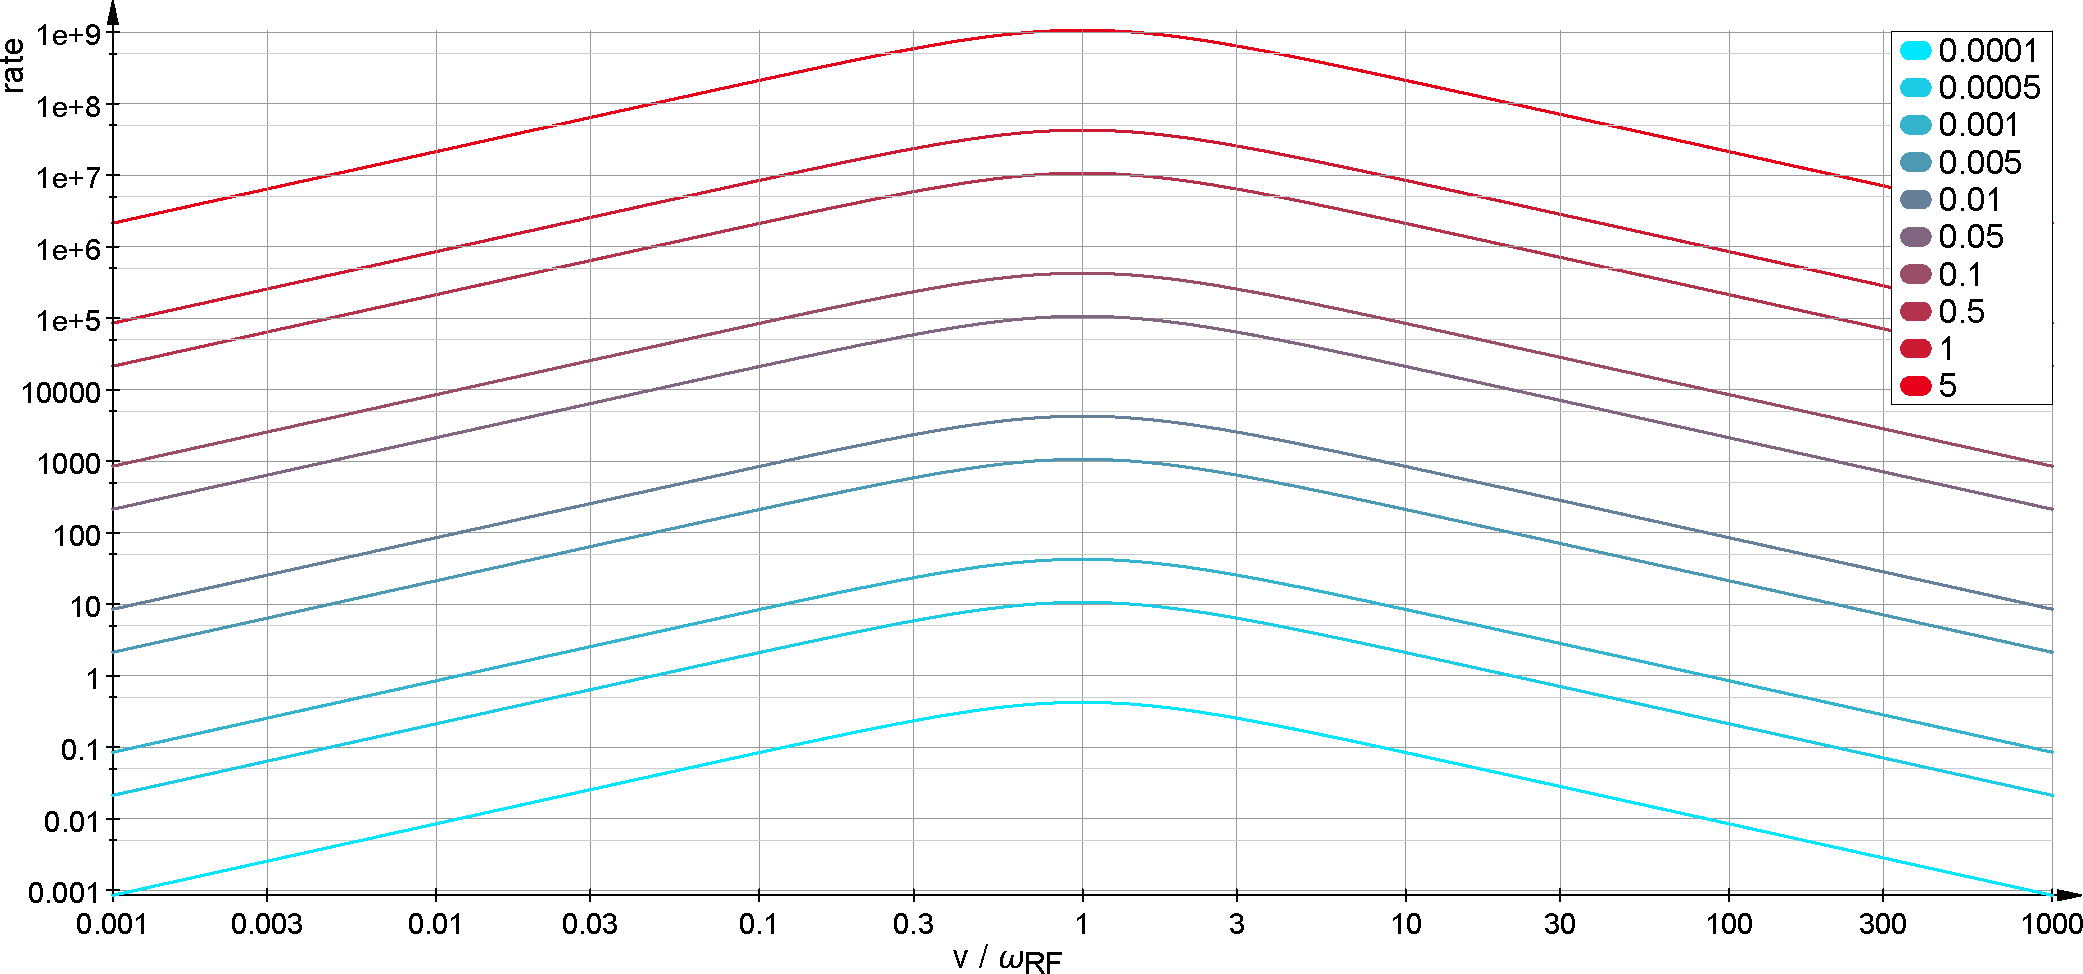
\includegraphics[width=1\columnwidth]{clipart/Ohmic-Heating}
\par\end{centering}
\caption{\label{fig:Energy-transfer-rate}Energy transfer rate in dependency
of $\nu/\omega_{\mathrm{applied}}$ (x-axis) and $\omega_{\mathrm{plasma}}/\omega_{\mathrm{applied}}$
(different curves).}
\end{figure}


\subsection{Stochastic}

The stochastic part of the dissipated power is difficult to calculate.
This power is consumed by the electrons colliding with the moving
sheath walls. Within the plasma bulk the electron distribution is
a \noun{Maxwell-Boltzmann} distribution but at the sheath borders
this is not the case because a fraction of the electrons are entering
the sheath and will be accelerated. It can even be shown (see \cite[sec. "Randschicht mit homogenem Ionendichteprofil"]{Keudell12})
that the assumption of a \noun{Maxwell-Boltzmann} distribution would
give that no power is dissipated but measurements show that power
is dissipated also at very low pressures (where ohmic dissipation
can be neglected). Finding an usable electron distribution is an active
research topic and an analytic solution nor a suitable approximation
has not yet been found.

\section{Electronegative Plasma}

Until now we assumed that all ions are positively charged because
each ionized atom or molecule looses one or more electrons. This is
correct in many cases but the electronegativity of oxygen and fluorine
is so high that the $\mathrm{O\cdot}$ and $\mathrm{F\cdot\,}$-radicals
can grab two or one electron, respectively. In this case we have also
a non-negligible amount of negatively charged ions. The density distributions
at a sheath in such an electronegative plasma is shown in \ref{fig:Scheme-electroneg-sheath}.
The negative ions are less mobile than the electrons and are therefore
pushed more away from the wall. As the result there is no clean sheath
border. However, we can define the sheath border at the largest $x$
at which $n_{i-}(x)+n_{e}(x)=n_{0}=n_{i+}(x)$ is fulfilled.

\begin{figure}[h]
\begin{centering}
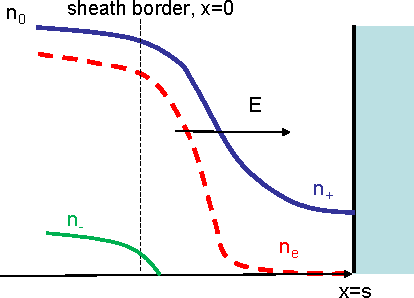
\includegraphics[width=0.5\columnwidth]{clipart/Electronegative-sheath-scheme}
\par\end{centering}
\caption{\label{fig:Scheme-electroneg-sheath}Scheme of the particle densities
in a sheath of an electronegative plasma. The wall is at $x=s$, the
sheath in the range $0\le x\le s$. Original image from \cite{Keudell12}.}
\end{figure}

In this case the \noun{Gauss} law needs to be modified and is instead
of (\ref{eq:Gauss-law1})
\begin{equation}
\frac{\mathrm{d}^{2}\Phi(x)}{\mathrm{d}x^{2}}=\frac{e}{\epsilon_{0}}\left(n_{e}(x)+n_{i-}(x)-n_{i+}(x)\right)
\end{equation}
with $\alpha=\cfrac{n_{i-}}{n_{e}}$ and $\beta=\cfrac{T_{e}}{T_{i}}$
we can solve this and get
\begin{equation}
v_{B}=\sqrt{\frac{k_{B}T_{e}}{M}\,\frac{1+\alpha}{1+\alpha\beta}}
\end{equation}
see \cite[sec. "Raumladungszone eines elektronegativen Plasmas"]{Keudell12}
for a detailed derivation.

In our applications we can assume that the electron temperature is
much higher than the temperature of the ions ($\beta\gg1$). In an
oxygen plasma we have $\alpha>0$. The dependence of $\alpha$ on
$v_{B}$ of an oxygen plasma is shown in \ref{fig:v_B-oxygen}.

\begin{figure}[h]
\begin{centering}
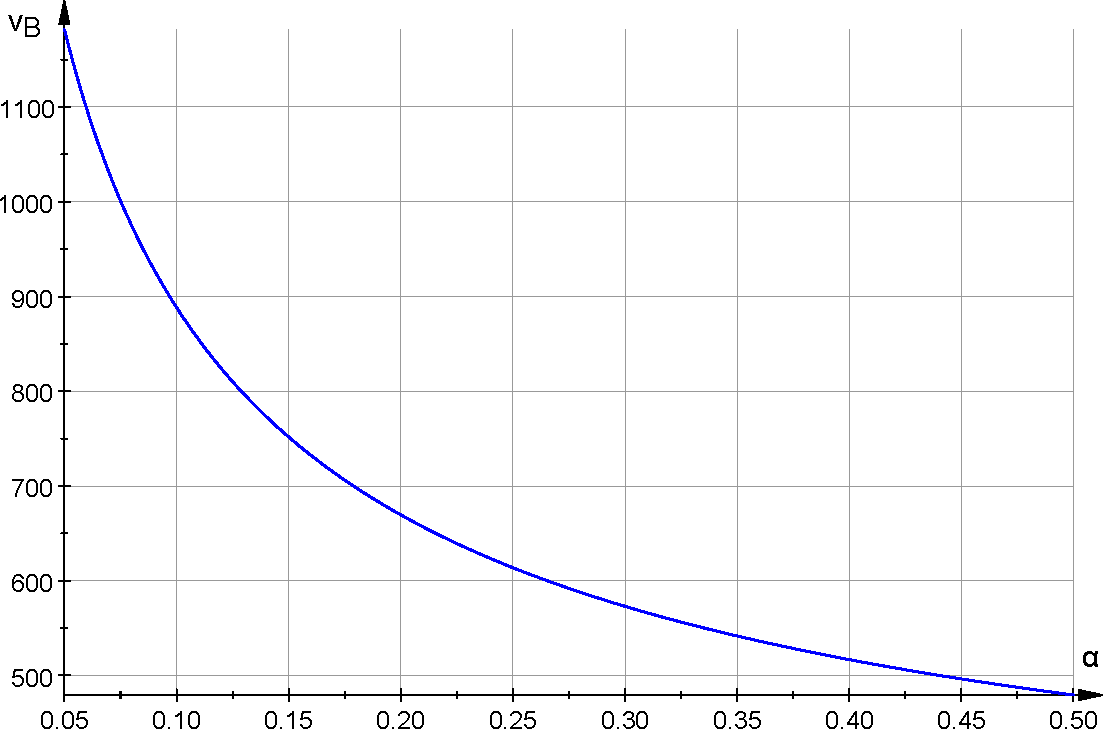
\includegraphics[width=0.6\columnwidth]{clipart/Bohm-oxygen}
\par\end{centering}
\caption{\label{fig:v_B-oxygen}$v_{B}$ in m/s for an oxygen plasma with a
non-negligible fraction of $\ce{O2-}$-ions ($M=32\,$u) in dependence
of the ion electronegativity $\alpha=\cfrac{n_{i-}}{n_{e}}$. $\beta$
was set to $\cfrac{T_{e}}{T_{i}}=\cfrac{3.48\cdot10^{4}}{300}=116$.}
\end{figure}

If we use this Bohm velocity in (\ref{eq:n_i}) we get instead of
(\ref{eq:Gauss-law2})
\begin{eqnarray}
\frac{\mathrm{d}E}{\mathrm{d}x} & = & =\cfrac{e\,n_{0}\,\sqrt{\frac{k_{B}T_{e}}{M}\,\frac{1+\alpha}{1+\alpha\beta}}}{\epsilon_{0}\,\sqrt{\frac{e\lambda}{M}\,E}}\nonumber \\
\epsilon_{0}\sqrt{E}\,\mathrm{d}\,E & = & e\,n_{0}\,\sqrt{\cfrac{k_{B}T_{e}}{e\lambda}\,\frac{1+\alpha}{1+\alpha\beta}}\,\mathrm{d}\,x\nonumber \\
E(x)^{3} & = & \frac{9}{4}\,n_{0}^{2}s^{2}\,\cfrac{ek_{B}T_{e}}{\epsilon_{0}^{2}\lambda}\,\frac{1+\alpha}{1+\alpha\beta}
\end{eqnarray}
with $E(s)=\cfrac{U}{s}$ we get
\begin{equation}
s=\left(\frac{4U^{3}\epsilon_{0}^{2}\lambda}{9n_{0}^{2}ek_{B}T_{e}}\,\frac{1+\alpha\beta}{1+\alpha}\right)^{1/5}
\end{equation}


\subsection*{Conclusion}

With a higher level of electronegativity the \noun{Bohm} velocity
is decreased. This increases the sheath thickness and therefore also
the sheath voltage, see the approximation (\ref{eq:U-sheath-approx}).

\newpage{}

\section{Energy of Impinging Ions}

Depending on the substrate it is important to know the energy of the
ions impinging the surface. For example for polymer substrates one
might estimate what chemical bonds can be cracked by impinging ions.

In the plasma bulk the ions have the Bohm velocity $v_{B}$, across
the sheath of the electrode there is a mean voltage of $U_{\mathrm{bias}}$
along the sheath thickness $s$. If the substrate is within the plasma
bulk the ions are accelerated by the floating potential $\Phi_{\mathrm{float}}$.
To calculate the ion energies we start with the time-independent equation
of motion:
\begin{equation}
M\ddot{x}=eE_{0}
\end{equation}
The sheath can be treated as parallel plate capacitor so that we have
$E_{0}=\cfrac{U_{\mathrm{bias}}}{s}$
\begin{equation}
M\ddot{x}=\frac{eU_{\mathrm{bias}}}{s}
\end{equation}

With the knowledge that the ions enter the sheath with the Bohm velocity
${\displaystyle v_{B}}=\sqrt{\cfrac{k_{B}T_{e}}{M}}$ the integration
gives 
\begin{eqnarray}
\dot{x}(t) & = & \frac{eU_{\mathrm{bias}}}{sM}\,t+C\\
\dot{x}(t=0) & = & v_{B}=C\\
\dot{x}(t) & = & \frac{eU_{\mathrm{bias}}}{sM}\,t+v_{B}\label{eq:x-punkt}
\end{eqnarray}
The further integration gives
\begin{equation}
x(t)=\frac{eU_{\mathrm{bias}}}{2sM}\,t^{2}+v_{B}t
\end{equation}

The acceleration only happens along the sheath thickness $s$. The
time of the acceleration is therefore
\begin{eqnarray}
s & = & \frac{eU_{\mathrm{bias}}}{2sM}\,\tau^{2}+v_{B}\tau\\
0 & = & \tau^{2}+\frac{2sv_{B}M}{eU_{\mathrm{bias}}}\tau-\frac{2s^{2}M}{eU_{\mathrm{bias}}}\\
\tau_{1,\,2} & = & -\,\frac{sv_{B}M}{eU_{\mathrm{bias}}}\pm\sqrt{\left(\frac{sv_{B}M}{eU_{\mathrm{bias}}}\right)^{2}+\frac{2s^{2}M}{eU_{\mathrm{bias}}}}
\end{eqnarray}

The time cannot be negative so that the solution is
\begin{eqnarray}
\tau & = & -\,\frac{sv_{B}M}{eU_{\mathrm{bias}}}+\sqrt{\left(\frac{sv_{B}M}{eU_{\mathrm{bias}}}\right)^{2}+\frac{2s^{2}M}{eU_{\mathrm{bias}}}}\nonumber \\
 & = & -\,\frac{sv_{B}M}{eU_{\mathrm{bias}}}+\frac{sM}{eU_{\mathrm{bias}}}\,\sqrt{v_{B}^{2}+\frac{2eU_{\mathrm{bias}}}{M}}\nonumber \\
 & = & \frac{sM}{eU_{\mathrm{bias}}}\left(-v_{B}+\sqrt{v_{B}^{2}+\frac{2eU_{\mathrm{bias}}}{M}}\right)
\end{eqnarray}

Putting this into (\ref{eq:x-punkt}) leads to the final velocity
of the ions
\begin{eqnarray}
v=\dot{x}(\tau) & = & \frac{eU_{\mathrm{bias}}}{sM}\,\frac{sM}{eU_{\mathrm{bias}}}\left(-v_{B}+\sqrt{v_{B}^{2}+\frac{2eU_{\mathrm{bias}}}{M}}\right)+v_{B}\nonumber \\
 & = & \sqrt{v_{B}^{2}+\frac{2eU_{\mathrm{bias}}}{M}}=\sqrt{\frac{k_{B}T_{e}+2eU_{\mathrm{bias}}}{M}}
\end{eqnarray}

We can now calculate the kinetic energy of the impinging ions:
\begin{eqnarray}
E_{\mathrm{kin}} & = & \frac{M}{2}v^{2}\nonumber \\
 & = & \frac{k_{B}T_{e}}{2}+eU_{\mathrm{bias}}
\end{eqnarray}
Taking into account that the ions can have more than one elementary
charge, we get with the number of elementary charges $\tilde{N}$
\begin{equation}
E_{\mathrm{kin}}=\frac{k_{B}T_{e}}{2}+\tilde{N}eU_{\mathrm{bias}}
\end{equation}

We cannot (yet) measure $T_{e}$ and therefore assume a typical temperature
of $T_{e}=3.5\cdot10^{4}\,$K we get with $\tilde{N}=1$
\begin{equation}
E_{\mathrm{impinge\,electrode}}=1.5+U_{\mathrm{bias}}\,\mathrm{eV}
\end{equation}

As the biases are in the range of several 100\,V, the influence of
the electron temperature can be neglected.

\bigskip{}

For the case that the substrate is on floating potential we have according
to (\ref{eq:Phi_float})
\begin{eqnarray}
E_{\mathrm{impinge\,floating}} & = & -\tilde{N}e\Phi_{\mathrm{float}}\nonumber \\
 & = & -\tilde{N}k_{B}T_{e}\ln\left(\frac{A_{w}+A_{e}}{A_{w}}\,\sqrt{\frac{2\pi m_{e}}{M}}\right)
\end{eqnarray}


\subsection*{Example}

For an Argon plasma ($M=40\,$u and $\tilde{N}=1$) in a typical setup
($A_{w}/A_{e}=6$) we have according to (\ref{eq:Phi_float}) $\Phi_{\mathrm{float}}=-13.5\,$V
and therefore $E_{\mathrm{impinge\,floating}}=13.5\,$eV.

\subsection*{Conclusions}

We see again that without measuring the electron temperature $T_{e}$
we cannot calculate the ion energies impinging substrates on floating
potential. In contrary for the energy of ions impinging substrates
on electrode potential the electron temperature can be neglected.

\section{Hollow Cathode Effect\label{sec:Hollow-cathode-effect}}

Plasmas with a high density are often observed within recessed volumes
like flanges or holes. Their occurrence can be explained geometrically.
Taking for example a hole with the radius $r$, a dense plasma will
burn in there if 
\begin{equation}
2s>r>s\label{eq:r-sheath-hollow}
\end{equation}
whereas $s$ is the thickness of the sheath. The reason is that the
ions impinging the wall generate secondary electrons. They are reflected
by the currently negatively charged walls and are accelerated so that
they can reach the opposite sheath. There they will again be reflected
because of the sheath potential. If both sheath borders are geometrically
close together, the electrons can therefore not leave the plasma but
will be reflected again and again. This increases the ionization rate
enormously because every additional electron can induce an ionization.\footnote{The effect of increasing the ionization rate by holding the electrons
in the plasma is also used by the magnetron setup in sputter devices,
where the electrons are kept by magnetic field lines.} The effect is illustrated in \ref{fig:Sketch-hole-setup}. It does
not usually not occur in holes in substrates at floating potential
because the floating potential is much lower than the bias voltage
and the holes are in most cases open so that the number of reflections
are low until the electrons can leave the hole volume.

\begin{figure}[h]
\begin{centering}
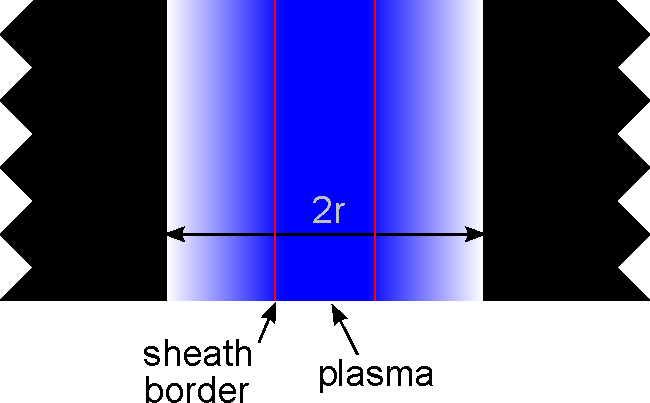
\includegraphics[width=0.55\columnwidth]{clipart/Hollow-cathode-scheme}
\par\end{centering}
\caption{\label{fig:Sketch-hole-setup}Sketch of a plasma in a hole with the
diameter $2r$. The borders of the sheath are so close together that
electrons will be reflected directly to the opposite sheath border
and therefore remain a long time in the hole resulting in a high ionization
rate.}
\end{figure}

We can assume that if $r<s$ no plasma will burn in the holes because
then no sheath can be formed. The factor~2 in (\ref{eq:r-sheath-hollow})
is an empirical value. If $r\gg s$ the sheath borders are too far
away to get the reflecting effect. The electrons are then not directly
reflected to the opposite sheath. So the hollow cathode effect only
exists for hole radiuses close above the sheath thickness.

\subsection*{Example}

A part should be coated at a constant pressure $p$ at a fixed bias
of $U_{\mathrm{bias,\thinspace1}}$ and later with a lower bias $U_{\mathrm{bias,\thinspace2}}$.
The values for $A_{e}$ and $A_{w}$ are known. In a preliminary test
one can measure the dissipated powers $P_{\mathrm{measured}}$ at
the given bias voltages.

The sheath thickness $s$ can be calculated using the approximation
(\ref{eq:s-approx}). Looking at (\ref{eq:U-matrix-relation}) and
(\ref{eq:U-sheath-approx}) we see that
\begin{equation}
\bar{s}_{e\,\mathrm{matrix}}^{2}=\bar{s}_{\mathrm{matrix}}^{2}\,\left(\frac{A_{w}}{A_{e}}\right)^{2}
\end{equation}
Using (\ref{eq:s-approx}) we can write
\begin{equation}
\bar{s}_{e\,\mathrm{matrix}}=\frac{I_{\mathrm{RF}}}{e\,n_{0}A_{w}\,\omega_{\mathrm{RF}}}\,\frac{A_{w}}{A_{e}}
\end{equation}
putting this into (\ref{eq:I_RF-approx}) gives
\begin{eqnarray}
\bar{s}_{e\,\mathrm{matrix}} & = & \frac{1}{e\,n_{0}A_{w}\,\omega_{\mathrm{RF}}}\,\frac{A_{w}}{A_{e}}\,\left(A_{e}\,\omega_{\mathrm{RF}}\right)^{2/3}\,\left(\frac{2\epsilon_{0}en_{0}P_{\mathrm{measured}}}{1.146}\right)^{1/3}\nonumber \\
 & = & \left(A_{e}\,\omega_{\mathrm{RF}}\right)^{-1/3}\,\left(en_{0}\right)^{-2/3}\,\left(\frac{2\epsilon_{0}P_{\mathrm{measured}}}{1.146}\right)^{1/3}
\end{eqnarray}
putting now (\ref{eq:n_0-approx}) into this leads to
\begin{eqnarray}
\bar{s}_{e\,\mathrm{matrix}} & = & \left(A_{e}\,\omega_{\mathrm{RF}}\right)^{-1/3}\,\left(\frac{e}{2e\epsilon_{0}U_{\mathrm{bias}}^{3}}\,\left(\frac{P_{\mathrm{measured}}}{1.146\cdot A_{e}\,\omega_{\mathrm{RF}}}\right)^{2}\left(\frac{A_{w}}{A_{e}}\right)^{6}\right)^{-2/3}\,\left(\frac{2\epsilon_{0}P_{\mathrm{measured}}}{1.146}\right)^{1/3}\nonumber \\
 & = & \frac{2.292\,\epsilon_{0}\,\omega_{\mathrm{RF}}\,A_{e}^{5}\,U_{\mathrm{bias}}^{2}}{P_{\mathrm{measured}}\,A_{w}^{4}}
\end{eqnarray}
We see that due to the matrix model, the mean free path $\lambda$
of the used precursor(s) and thus the pressure does not have an influence
on the approximated sheath thickness.

To calculate the minimal hole radius, we use the lower bias and get
$\bar{s}_{e\,\mathrm{matrix\,min}}$. The maximal sheath thickness
$\bar{s}_{e\,\mathrm{matrix\,max}}$ is calculated using the larger
bias. According to (\ref{eq:r-sheath-hollow}) only in holes with
a radius in the range of $2\bar{s}_{e\,\mathrm{matrix\,max}}>r>\bar{s}_{e\,\mathrm{matrix\,min}}$
the hollow cathode effect will occur.

\begin{lyxgreyedout}
Note that for conductive substrates the electrode area is the uncovered
surface area of the electrode plus the visible surface area of the
substrate. For non conductive substrates the electrode area is only
the uncovered surface area of the electrode.%
\end{lyxgreyedout}

In practice there are often have setups like the one that is schematically
shown in \ref{fig:Scheme-holder}. One uses then a substrate holder
that reduces the gap to the substrates so that no dense plasma will
burn in. With (\ref{eq:s_precise}) we are able to calculate the required
gap.

\begin{figure}[h]
\begin{centering}
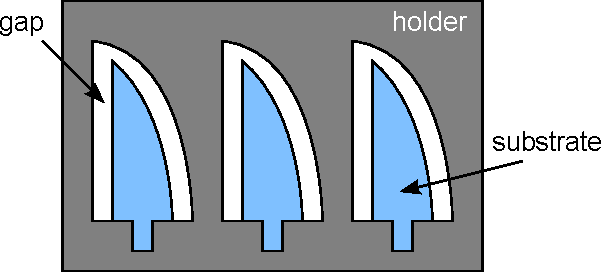
\includegraphics[width=0.6\columnwidth]{clipart/Substrate-holder-example}
\par\end{centering}
\caption{\label{fig:Scheme-holder}Scheme of a typical sample holder used to
coat e.\,g. knife blades.}
\end{figure}

\newpage{}

\section{Conclusions}

We see that with the knowledge of the plasma input power $P_{\mathrm{measured}}$,
the bias voltage $U_{\mathrm{bias}}$ and the electron temperature
$T_{e}$ we are able to explain what is happening in a CCP. But as
long as we do not measure $T_{e}$ we cannot calculate exact values
although this is often necessary, e.g. to avoid the hollow cathode
effect. We need $T_{e}$ to be able to calculate
\begin{itemize}
\item the sheath thickness $s$, see (\ref{eq:s_e-mean}) -- necessary
to calculate the diameter of holes in which the hollow cathode effect
will occur
\item the voltage across a sheath, see (\ref{eq:U_w-precise}) -- necessary
to calculate plasma density and thus the ionization ratio, see (\ref{eq:ionization-ratio})
\item the floating potential $\Phi_{\mathrm{floating}}$, see (\ref{eq:Phi_float})
-- necessary to calculate the energy of ions impinging substrates
in the plasma bulk
\end{itemize}

\appendix

\section{Mean Free Paths\label{sec:Mean-Free-Paths}}

The mean free paths $\lambda$ given here were calculated using the
ideal gas law and thus this formula:
\begin{equation}
\lambda=\frac{k_{\mathrm{B}}T}{\sqrt{2}\pi d^{2}p}
\end{equation}
where $k_{\mathrm{B}}=1.38\cdot10^{-23}$\,J/K is the \noun{Boltzmann}
constant, $T$ the temperature in Kelvin, $p$ the pressure in Pascal
and $d$ the largest diameter of the moelcule in meters.

\textbf{Note:} the $\lambda$ listed in \ref{tab:Mean-free-paths}
are according to $T=298\,K$ and $p=1$\,Pa. For other pressures,
the value can be divided by the actual pressure.

The molecule diameter was determined using the program \textsf{\href{https://avogadro.cc/}{Avogadro}}
by optimizing its geometry in 5000~steps using the \href{https://en.wikipedia.org/wiki/Merck_molecular_force_field}{Merck molecular force field}
method 94 (MMFF94). The largest molecule diameter was measured out
using the calculated coordinates of the hydrogen molecules the most
far away from each other. For hydrogen-free molecules, the atom ccordinates
were used plus 2\,times the \href{http://en.wikipedia.org/wiki/Atomic_radius}{atomic radius}
of the outermost atoms. Despite that this method is not very precise,
it delivers realistic $\lambda$ for practical use,

\textbf{Keep in mind}, that the $\lambda$ given in \ref{tab:Mean-free-paths}
are only usable for complete molecules. As soon as a molecule is cracked
in the plasma or reacted, its geometry has changed fundamentally and
calculations using specific $\lambda$ are not sensible.

\begin{table}[!h]
\begin{centering}
\caption{\label{tab:Mean-free-paths}Mean free paths $\lambda$ for some molecules,
commonly used in PE-CVD processes; for $T=298\,K$ and $p=1$\,Pa.}
\par\end{centering}
\centering{}%
\begin{tabular}{cc}
\toprule 
Molecule & $\lambda$ in mm\tabularnewline
\midrule
\midrule 
\multicolumn{2}{c}{Gases}\tabularnewline
\midrule 
\href{https://en.wikipedia.org/wiki/Acetylene}{Acetylene} & 8.4\tabularnewline
\midrule 
\href{https://en.wikipedia.org/wiki/Ammonia}{Ammonia} & 35.3\tabularnewline
\midrule 
\href{http://en.wikipedia.org/wiki/Argon}{Argon} & 17.9\tabularnewline
\midrule 
\href{https://en.wikipedia.org/wiki/Carbon_tetrafluoride}{Carbon tetrafluoride} & 8.9\tabularnewline
\midrule 
\href{https://en.wikipedia.org/wiki/Hydrogen}{Hydrogen} & 92.6\tabularnewline
\midrule 
\href{http://en.wikipedia.org/wiki/Methane}{Methane} & 29.2\tabularnewline
\midrule 
\href{https://en.wikipedia.org/wiki/Nitrogen}{Nitrogen} & 13.7\tabularnewline
\midrule 
\href{https://en.wikipedia.org/wiki/Nitrous_oxide}{Nitrous oxide} & \tabularnewline
Constitution $\ce{N\tbond N-O}$ & 6.2\tabularnewline
Constitution $\ce{N\dbond N\dbond O}$ & 6.6\tabularnewline
\midrule 
\href{https://en.wikipedia.org/wiki/Oxygen}{Oxygen} & 16.1\tabularnewline
\midrule
\midrule 
\multicolumn{2}{c}{Precursors}\tabularnewline
\midrule 
\href{http://www.chemspider.com/Chemical-Structure.56117.html}{Dimethyldiethoxysilane} & 2.1\tabularnewline
\midrule 
\href{http://www.chemspider.com/Chemical-Structure.59573.html}{Dimethyldimethoxysilane} & 1.1\tabularnewline
\midrule 
\href{http://de.wikipedia.org/wiki/Hexamethyldisilazan}{Hexamethyldisilazan} & 1.6\tabularnewline
\midrule 
\href{https://en.wikipedia.org/wiki/Hexamethyldisiloxane}{Hexamethyldisiloxane} & 1.6\tabularnewline
\midrule 
\href{https://en.wikipedia.org/wiki/Hexane}{Hexane} & 1.4\tabularnewline
\midrule 
\href{http://www.chemspider.com/Chemical-Structure.13803.html}{Methyltrimethoxysilane} & 2.0\tabularnewline
\midrule 
\href{https://en.wikipedia.org/wiki/Tetraethyl_orthosilicate}{Tetraethylorthosilikate} & 1.1\tabularnewline
\midrule 
\href{http://www.chemspider.com/Chemical-Structure.10654696.html}{Tetramethyldisilazane} & 1.7\tabularnewline
\midrule 
\href{http://www.chemspider.com/Chemical-Structure.17619.html}{Tetramethyldisiloxane} & 1.7\tabularnewline
\midrule 
\href{https://en.wikipedia.org/wiki/Tetramethylsilane}{Tetramethylsilane} & 3.9\tabularnewline
\midrule 
\href{http://www.chemspider.com/Chemical-Structure.68503.html}{Vinyltrimethoxysilane} & 2.3\tabularnewline
\bottomrule
\end{tabular}
\end{table}

\newpage{}

\bibliographystyle{IEEEtran}
\bibliography{biblio/Plasma}

\end{document}
